% THIS DOCUMENT IS FOLLOWS THE VOLERE TEMPLATE BY Suzanne Robertson and James Robertson
% ONLY THE SECTION HEADINGS ARE PROVIDED
%
% Initial draft from https://github.com/Dieblich/volere
%
% Risks are removed because they are covered by the Hazard Analysis
\documentclass[12pt]{article}
\pdfinfoomitdate=1
\pdftrailerid{}

\usepackage{booktabs}
\usepackage{tabularx}
\usepackage{hyperref}
\usepackage{enumitem}
\hypersetup{
    bookmarks=true,         % show bookmarks bar?
    colorlinks=true,        % false: boxed links; true: colored links
    linkcolor=red,          % color of internal links (change box color with linkbordercolor)
    citecolor=green,        % color of links to bibliography
    filecolor=magenta,      % color of file links
    urlcolor=cyan           % color of external links
}
\usepackage{float}
\usepackage{makecell}
\usepackage[table]{xcolor}
\usepackage{array} % for \newcolumntype

% Example custom columns (centered/left X variants)
\newcolumntype{Y}{>{\centering\arraybackslash}X}
\newcolumntype{Z}{>{\raggedright\arraybackslash}X}


\newcommand{\lips}{\textit{Insert your content here.}}

%% Comments

\usepackage{color}

% \newif\ifcomments\commentstrue %displays comments
\newif\ifcomments\commentsfalse %so that comments do not display

\ifcomments
  \newcommand{\authornote}[3]{\textcolor{#1}{[#3 ---#2]}}
  \newcommand{\todo}[1]{\textcolor{red}{[TODO: #1]}}
\else
  \newcommand{\authornote}[3]{}
  \newcommand{\todo}[1]{}
\fi

\newcommand{\wss}[1]{\authornote{magenta}{SS}{#1}}
\newcommand{\plt}[1]{\authornote{cyan}{TPLT}{#1}} %For explanation of the template
\newcommand{\an}[1]{\authornote{cyan}{Author}{#1}}

%% Common Parts

\newcommand{\progname}{RoCam} % PUT YOUR PROGRAM NAME HERE
\newcommand{\authname}{Team \#3, SpaceY
    \\ Zifan Si
    \\ Jianqing Liu
    \\ Mike Chen
    \\ Xiaotian Lou} % AUTHOR NAMES                  

\usepackage{hyperref}
\hypersetup{colorlinks=true, linkcolor=blue, citecolor=blue, filecolor=blue,
    urlcolor=blue, unicode=false}
\urlstyle{same}

\usepackage{indentfirst}
\usepackage{graphicx}

\usepackage{titling}

\pretitle{\begin{center}
\includegraphics[width=0.5\textwidth]{../../assets/logo/black.png}\\[0.75em]\LARGE}
        \posttitle{\par\end{center}}

\usepackage[letterpaper, portrait, margin=1in]{geometry}

\usepackage{placeins}

\begin{document}

\title{Software Requirements Specification for \progname: High Performance Vision-Guided Rocket Tracker}
\author{\authname}
\date{\today}

\maketitle

~\newpage

\tableofcontents

~\newpage

\section*{Revision History}

\begin{tabularx}{\textwidth}{p{3cm}p{2cm}X}
  \toprule {\textbf{Date}} & {\textbf{Version}} & {\textbf{Notes}} \\
  \midrule
  Date 1                   & 1.0                & Notes            \\
  Date 2                   & 1.1                & Notes            \\
  \bottomrule
\end{tabularx}

~\\

~\newpage
\section{Purpose of the Project}
\subsection{User Business}

Student and amateur rocketry teams, launch organizers, and technical judges
need reliable, high-fidelity visual evidence of rocket flights to analyze
staging behavior, parachute deployment, and flight anomalies that occur at
extreme speeds and altitudes. Manual camera operation is impractical in these
conditions, and existing tools (manual PTZ/GPS-centric systems) often fail to
maintain visual lock on small, fast-moving vehicles. This project addresses
this gap with an autonomous, vision-based tracking camera designed to lock onto
and follow rockets from launch through landing, providing real-time and
recorded footage for post-flight analysis and event operations.

\subsection{Goals of the Project}

\textbf{Purpose:}

Develop a software+hardware stack (the system) that is able to command a gimbal
with a camera mounted on it to track and record model rocket launches.

\textbf{Advantage:}

The system provides insights into the flight performance by having high quality
flight footage.

\textbf{Measure:}

Deploy the system at small-scale model rocket launch site with apogee less than
200 meters. The system should provide higher quality flight footage than the
manual camera operation.

\section{Stakeholders}

\subsection{Client}

The client of this project is McMaster Rocketry Team. they are the primary end
users who will deploy the system during launches.

\subsection{Customer}

Apart from our client, we also identified the following customers that may be
interested in using the project:

\begin{enumerate}
  \item \textbf{Model Rocketry Event Organizers}: Benefit from
        reliable tracking for live streaming of rocket flights.
  \item \textbf{Model Rocketry Safety Officers}: Benefit from
        live monitoring of parachute deployment and landing location
        of the rockets.
  \item \textbf{Aerospace Engineers and Researchers}: Benefit from
        high-quality flight footage to validate models, improve rocket
        designs, and support experimental research.
\end{enumerate}

\subsection{Other Stakeholders}

\begin{enumerate}
  \item \textbf{Dr. Shahin Sirouspour (Supervisor)}: Provides
        technical guidance, project oversight, and mentorship. Ensures
        the project aligns with academic standards, engineering best
        practices, and capstone deliverable expectations.
\end{enumerate}

\subsection{Hands-On Users of the Project}

Here are the users that will be interacting with the product directly.

\textbf{Role: Camera Operator}

The camera operator controls the system through the UI, starts/stops
recordings, manages tracking states, and monitors preview. The camera operator
is assumed to have a decent level of familiarity with technology, and have been
trained on the use of the product.

\textbf{Role: Live Stream Technician}

The live stream technician manages the video feed from the system to the live
streaming equipments. The live stream technician is assumed to have a high
level of familiarity with live streaming software and hardware.

\textbf{Role: Flight Performance Analyst}

The flight performance analyst is a member of the rocketry team that
reconstructs flight profiles from sensor data and camera footage to understand
how the rocket behaves during ascent and descent. The flight performance
analyst is assumed to have a high level of familiarity with rocket flight
dynamics and software used for analysis.

\textbf{Role: Live Stream / Recordings Viewers}

People who view the live stream or recorded videos. They can be anyone from the
general public that are interested in the launch, or the team members
themselves. They are assumed to have a basic level of familiarity with
technology.

\subsection{Personas}

\subsubsection*{Alexis Andrade}

\textbf{Age}: 28

\textbf{Role}: Camera Operator

Alexis works as an industrial automation technician in Hamilton, Ontario, where
she designs and maintains robotic assembly systems for a manufacturing firm.
Outside of work, her real passion lies in high-speed imaging and experimental
photography — a hobby that naturally led her to volunteer as a staff camera
operator at university rocketry competitions. She loves the mix of engineering
precision and adrenaline that comes with capturing a successful rocket launch.

She lives with her partner and their energetic border collie, Pixel. Alexis
spends her weekends hiking the Bruce Trail, refurbishing vintage lenses, or
volunteering at local maker fairs. Her favorite food is falafel, and she always
packs a thermos of strong coffee for early launch mornings. She listens to
synthwave and retro electronic music on long drives to test sites, finding it
helps her stay calm and focused.

Alexis is confident with technology but prefers systems that are reliable and
straightforward. She values hands-on work, hates clunky software interfaces,
and believes in simplicity over flashiness. “If I need a manual,” she likes to
say, “the interface is wrong.” Her cool temperament and technical precision
make her a trusted member of the launch operations crew.

\subsubsection*{Brandon Brooks}

\textbf{Age}: 23

\textbf{Role}: Flight Performance Analyst

Brandon is in his final year of mechanical engineering at a Canadian university
and serves as a flight performance analyst for his rocketry team. His specialty
is reconstructing flight profiles from sensor data and camera footage to
understand how the rocket behaves during ascent and descent. He joined the team
for the engineering challenge but stayed because he loves the mix of theory,
experimentation, and teamwork.

Originally from Calgary, Brandon now lives in a small off-campus apartment
filled with model rockets, whiteboards, and a curious cat named Fourier. He's
known for his patience and meticulous documentation — traits that make him the
go-to person for post-launch analysis. When he's not studying or coding MATLAB
scripts, he's cooking ramen, taking photos, or biking along Lake Ontario.

Brandon listens to ambient and post-rock while he works, loves strong coffee,
and dislikes chaotic testing days where data logging gets overlooked. His
attitude toward technology is analytical but practical: he values transparency,
well-documented systems, and data that “speaks for itself.” For him, every
successful flight is a story written in numbers and motion.

\subsubsection*{Christopher Chou}

\textbf{Age}: 59

\textbf{Role}: Event Organizer / Live Stream Technician

Christopher is a retired broadcast engineer who spent three decades working in
television production for CBC Toronto. After retirement, he moved to Burlington
and found a new passion in volunteer work, helping organize live streams and
event logistics for student rocketry competitions. For him, it's the perfect
blend of his lifelong love of broadcasting and his fascination with aerospace
technology.

He's married with two grown children who live abroad, and he often jokes that
the rocketry community has become his “third family.” Christopher loves cooking
Cantonese comfort food — especially steamed dumplings and congee — and enjoys
jazz and classic rock in equal measure. He spends his spare time restoring old
audio equipment, gardening, and taking long weekend drives along the Niagara
Escarpment.

Christopher's approach to technology is deeply pragmatic: he respects
automation but insists that every system should have a manual override. He
likes tidy wiring, clear documentation, and software that doesn't crash
midstream. He dislikes unnecessary complexity and “updates that fix what wasn't
broken.” To younger team members, he's both a mentor and the steady hand who
keeps the broadcast running when chaos hits.
\subsection{Priorities Assigned to Users}

\textbf{Key Users}: Camera Operator, Live Stream Technician

\textbf{Secondary User}: Flight Performance Analyst, Live Stream / Recordings Viewers, Event Organizer

\subsection{User Participation}

Through out the development process, the development team will continue to
iterate on the requirements based on feedback from these users:

\begin{enumerate}
  \item \textbf{Camera Operator}: At least three field tests will be conducted
        to gather feedback from the camera operator. Each field test will last
        half a day to a day.
  \item \textbf{Live Stream Technician}: At least two meetings will be conducted
        to gather feedback from the live stream technician.
\end{enumerate}

\subsection{Maintenance Users and Service Technicians}

Due to the nature of this project as a capstone requirement, there are
currently no expected maintenance users.

\section{Mandated Constraints}
\subsection{Solution Constraints}

\begin{itemize}[leftmargin=*]
  \item[SC-1] \emph{The system must use computer vision for rocket detection and
          tracking}\\[2mm]
        \textbf{Rationale:} There is already a camera connected to the system for recording, using computer vision for detection and tracking is the most efficient way to do it. \\
        \textbf{Fit Criterion:} The system should be able to detect and track a rocket based only on the camera feed.
\end{itemize}

\subsection{Implementation Environment of the Current System}

There are no constrains on the hardware platform the system need to use.

\subsection{Partner or Collaborative Applications}

The system is expected to be used with a gimbal with a camera mounted on it.
The system will command the gimbal to track and record model rocket launches.

\subsection{Off-the-Shelf Software}

There are no constrains on the off-the-shelf software the system need to use.

\subsection{Anticipated Workplace Environment}

The system should be designed to operate in a large-scale outdoor launch
environment, for example, the Launch Canada launch site in Timmins, Ontario, Or
Spaceport America in New Mexico.

The tracking camera will be operated at outdoor launch sites, typically in wide
open fields or designated rocket ranges. Launches occur only under clear, sunny
conditions with few or no clouds.

Additionally, users often wear hearing protection devices to mitigate high
acoustic noise from tools, filling tanks, and generators.

Launch sites are typically in a remote area, with limited or no internet
access.

\subsection{Schedule Constraints}

\begin{itemize}[leftmargin=*]
  \item[SHC-1] \emph{The project shall be completed by April 2026, with interim
          deadlines for key milestones such as Proof of Concept (November 2025) and the
          final demonstration (March 2026).}\\[2mm]
        \textbf{Rationale:} These deadlines are based on the academic timeline and the expectations of the capstone course.\\
        \textbf{Fit Criterion:} All project components must be completed and fully functional by the final demonstration in March 2026.
\end{itemize}

\subsection{Budget Constraints}

\begin{itemize}[leftmargin=*]
  \item[BC-1] \emph{The project shall not exceed the budget of 500CAD.}\\[2mm]
        \textbf{Rationale:} Limited by the capstone project requirement.\\
        \textbf{Fit Criterion:} The sum of the costs of the hardware components required for the project must be less than 500CAD.
\end{itemize}

\subsection{Enterprise Constraints}

\begin{itemize}[leftmargin=*]
  \item[EC-1] \emph{The product shall be built to comply with the standards of McMaster
          University's capstone project requirements and academic integrity policies.}\\[2mm]
        \textbf{Rationale:} The project is part of the university's curriculum and must adhere to its standards.\\
        \textbf{Fit Criterion:} The product must meet the requirements specified by the course syllabus and project advisor.
\end{itemize}

\section{Naming Conventions and Terminology}
\subsection{Glossary of All Terms, Including Acronyms, Used by Stakeholders
  involved in the Project}

\begin{enumerate}
  \item \textbf{The System}: The software+hardware stack developed for this project that is able to command a gimbal with camera mounted on it to track and record a rocket flight. (the gimbal and the camera are not a part of the system)
  \item \textbf{Gimbal}: A gimbal is a motorized device that rotates based on the commands sent to it.
  \item \textbf{Rocket}: Refers to a model rocket.
  \item \textbf{Ascent}: The stage in a model rocket flight where the rocket is ascending.
  \item \textbf{Descent}: The stage in a model rocket flight where the rocket has reached its apogee and is descending.
\end{enumerate}

\section{Relevant Facts And Assumptions}
\subsection{Relevant Facts}

None.

\subsection{Business Rules}

None.

\subsection{Assumptions}

\begin{itemize}[leftmargin=*]
  \item[AS-1] The system will not be connected to the public internet; thus, no
        authentication is required.
  \item[AS-2] The system will only be physically accessed by authorized personnel.
  \item[AS-3] Only one rocket will be flying at a time.
  \item[AS-4] The gimbal connected to the system has adequate performance to track the
        rocket (e.g., it can turn fast enough and has enough range of motion).
  \item[AS-5] 110V AC power is available at the launch site.
  \item[AS-6] It will always be sunny at the launch site, because the launch would be
        cancelled in case of bad weather.
\end{itemize}

\section{The Scope of the Work}
\subsection{The Current Situation}

Currently, the process of recording and analyzing rocket flights relies on
manual camera operators positioned at safe distances from the launch pad. These
operators attempt to visually follow the rocket during ascent and descent using
consumer or semi-professional video cameras mounted on tripods or pan-tilt
systems.

This approach suffers from several limitations:

\textbf{Accuracy:} Human reaction time and limited field of view make it nearly
impossible to keep fast-moving rockets (often exceeding Mach speeds) centered
in frame. The footage is frequently lost during liftoff or staging events,
leaving gaps in post-flight analysis.

\textbf{Safety Constraints:} Because a human operator must be physically present, camera
placement is restricted to safe zones, which may not provide optimal viewing
angles. Cameras cannot always be positioned where the best line-of-sight
exists.

\textbf{Operational Overhead:} Each launch requires trained operators, setup time, and
coordination with the launch control team. Fatigue, stress, and environmental
conditions (sun glare, wind, dust) further degrade performance.

\textbf{Data Quality:} The video produced by manual operators is often shaky,
inconsistently framed, and lacking synchronization with other flight data
(e.g., telemetry or gimbal angle). This reduces its value for engineering
analysis and competition reporting.

\subsection{The Context of the Work}

\hyperref[img:context-of-work]{Figure 1} identifies the scope of the
investigation necessary in order to discover the requirements related to the
work of tracking rockets. The model shows the detailed area of investigation
and how it connects to the adjacent systems.

\begin{figure}[H]
  \centering
  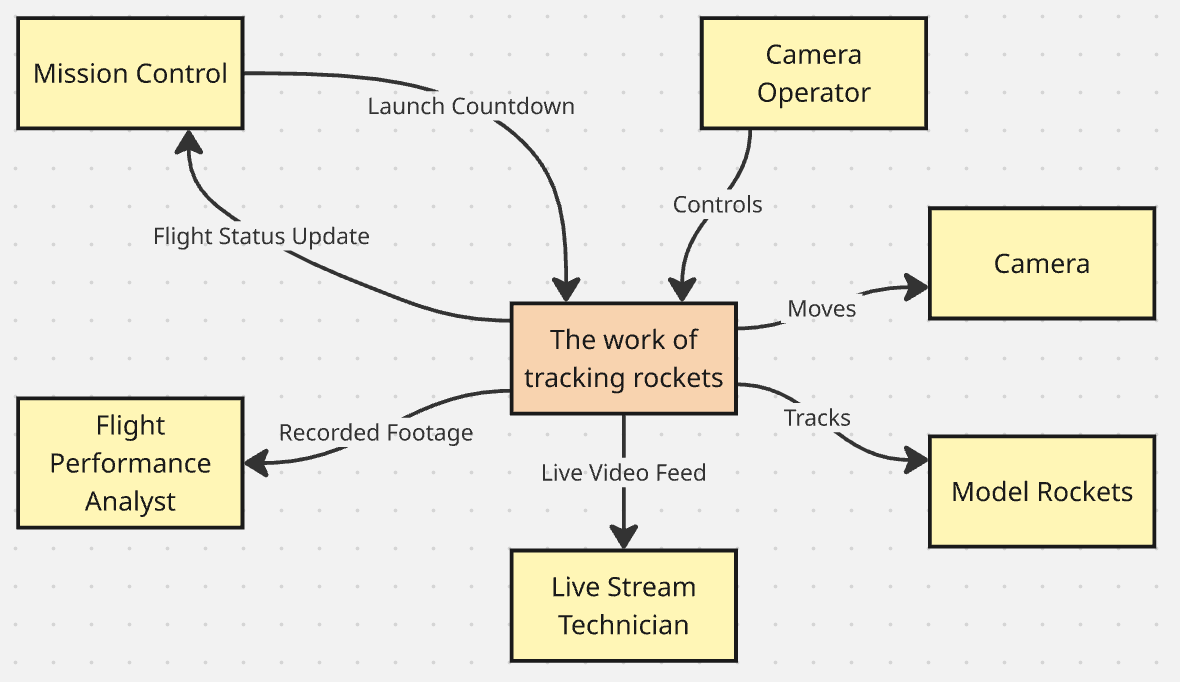
\includegraphics[width=\textwidth,height=\textheight,keepaspectratio]{../Images/context_of_work.png}
  \caption{Context of Work Diagram}
  \label{img:context-of-work}
\end{figure}

\subsection{Work Partitioning}

The \hyperref[tab:work-part]{Table 1} identifies all business events happening
in the real world that affect the work of tracking rockets.

\begin{table}[H]
  \centering
  \setlength\extrarowheight{5mm}
  \begin{tabularx}{\textwidth}{cp{1.5in}X}
    \toprule \textbf{No.} & \textbf{Event Name}                                  &
    \textbf{Input / Output}                                                        \\
    \midrule
    BUC 1                 & Output live video                                    &
    (in) Video feed from camera \newline
    (out) Transmitting the video to the live stream
    \\
    BUC 2                 & Launch countdown starts                              &
    (in) Vocal count down from Mission Control \newline
    (out) Start recording the rocket flight
    \\
    BUC 3                 & Rocket takes flight                                  &
    (in) Video feed from camera \newline
    (out) Keeps pointing the camera to the rocket
    \\
    BUC 4                 & Rocket completes flight                              &
    (in) Video feed from camera \newline
    (out) Stop tracking the rocket \newline
    (out) Save the video  \newline
    (out) Update mission control on flight status
    \\
    BUC 5                 & Flight performance analyst wants to view the footage &
    (in) Request from Flight performance analyst \newline
    (out) Exported video files and logs
    \\
    \bottomrule
  \end{tabularx}
  \caption{Work Partitioning of System}
  \label{tab:work-part}
\end{table}

\subsection{Specifying a Business Use Case (BUC)}

Each event listed in \hyperref[tab:work-part]{Table 1} is expanded into an
individual business use case (BUC) which describes business logic in detail.

~\\

\textbf{BUC 1: Output live video.}

\textbf{Trigger:} None, always active.

\textbf{Interested Stakeholders:} Model Rocketry Event Organizers

\textbf{Preconditions:} Camera is powered on.

\textbf{Main Flow of Steps:}
\begin{enumerate}
  \item The camera operator connect the camera to the live streaming equipments.
\end{enumerate}

\textbf{Outcome:} The live stream receives a video feed from the camera.

~\\

\textbf{BUC 2: Launch countdown starts.}

\textbf{Trigger:} Mission Control begins the countdown to launch.

\textbf{Interested Stakeholders:} Model Rocketry Event Organizers.

\textbf{Preconditions:} Camera is powered on and ready to record.

\textbf{Main Flow of Steps:}
\begin{enumerate}
  \item The camera operator points the camera to the rocket
  \item The camera operator starts recording.
\end{enumerate}

\textbf{Outcome:} Recording of the rocket flight is started.

~\\

\textbf{BUC 3: Rocket takes flight.}

\textbf{Trigger:} Rocket ignition and liftoff are observed.

\textbf{Interested Stakeholders:} Model Rocketry Event Organizers, Aerospace Engineers and Researchers.

\textbf{Preconditions:} Camera is pointing at the rocket and recording.

\textbf{Main Flow of Steps:}
\begin{enumerate}
  \item The camera operator keeps pointing the camera to the rocket.
  \item If the rocket stages, the camera operator points the camera to the next stage.
\end{enumerate}

\textbf{Outcome:} The camera remains pointed at the rocket throughout the flight.

~\\

\textbf{BUC 4: Rocket completes flight.}

\textbf{Trigger:} Rocket landing is observed.

\textbf{Interested Stakeholders:} Model Rocketry Event Organizers, Model Rocketry Safety Officers.

\textbf{Preconditions:} Camera is pointing at the rocket and recording.

\textbf{Main Flow of Steps:}
\begin{enumerate}
  \item The camera operator confirms end of flight based on callout or observation.
  \item The camera operator ends the recording.
  \item The camera operator stops pointing the camera to the rocket.
  \item The camera operator communicates the flight status to Mission Control.
\end{enumerate}

\textbf{Outcome:} Video and logs are safely stored and the flight status is communicated to Mission Control.

~\\

\textbf{BUC 5: Flight performance analyst wants to view the footage.}

\textbf{Trigger:} Flight performance analyst requests to view the footage.

\textbf{Interested Stakeholders:} Aerospace Engineers and Researchers.

\textbf{Preconditions:} None.

\textbf{Main Flow of Steps:}
\begin{enumerate}
  \item The flight performance analyst provides date and time of the flight.
  \item The camera operator looks up the flight in the database.
  \item If the flight is found, the camera operator exports the video files and logs.
  \item If the flight is not found, the camera operator informs the flight performance
        analyst that the flight is not found.
\end{enumerate}

\textbf{Outcome:} The flight performance analyst receives the video files and logs.

\section{Business Data Model and Data Dictionary}
\subsection{Business Data Model}

The business data model consists of a list of launches, and for each launch,
the video footage and logs associated with the launch.

\begin{figure}[H]
  \centering
  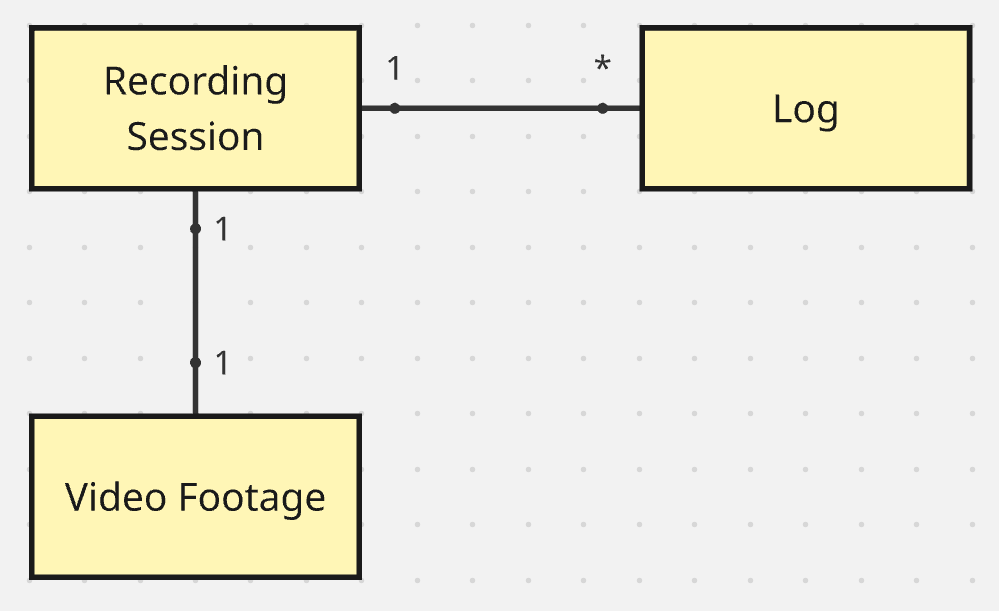
\includegraphics[width=\textwidth,height=\textheight,keepaspectratio]{../Images/business_data_model.png}
  \caption{Business Data Model}
  \label{img:business-data-model}
\end{figure}

\subsection{Data Dictionary}

\begin{table}[H]
  \centering
  \setlength\extrarowheight{5mm}
  \begin{tabularx}{\textwidth}{lXp{1in}}
    \toprule \textbf{Name} & \textbf{Content}               &
    \textbf{Type}                                             \\
    \midrule
    Recording Session      & date + time                    &
    Class
    \\
    Video Footage          & Recorded video from the camera &
    Class
    \\
    Log                    & timestamp + gimbal angle       &
    Class
    \\
    \bottomrule
  \end{tabularx}
  \caption{Data Dictionary}
  \label{tab:data-dictionary}
\end{table}

\section{The Scope of the Product}
\subsection{Product Boundary}

The product boundary defines which parts of the work are handled by the system
and which parts remain the responsibility of human actors.

In \hyperref[img:product-boundary]{Figure 3}, The product use cases (PUCs) are
the ellipses inside the boundary. Each PUC is labeled with one or more BUCs
that it came from.

\FloatBarrier
\begin{figure}[h]
  \centering
  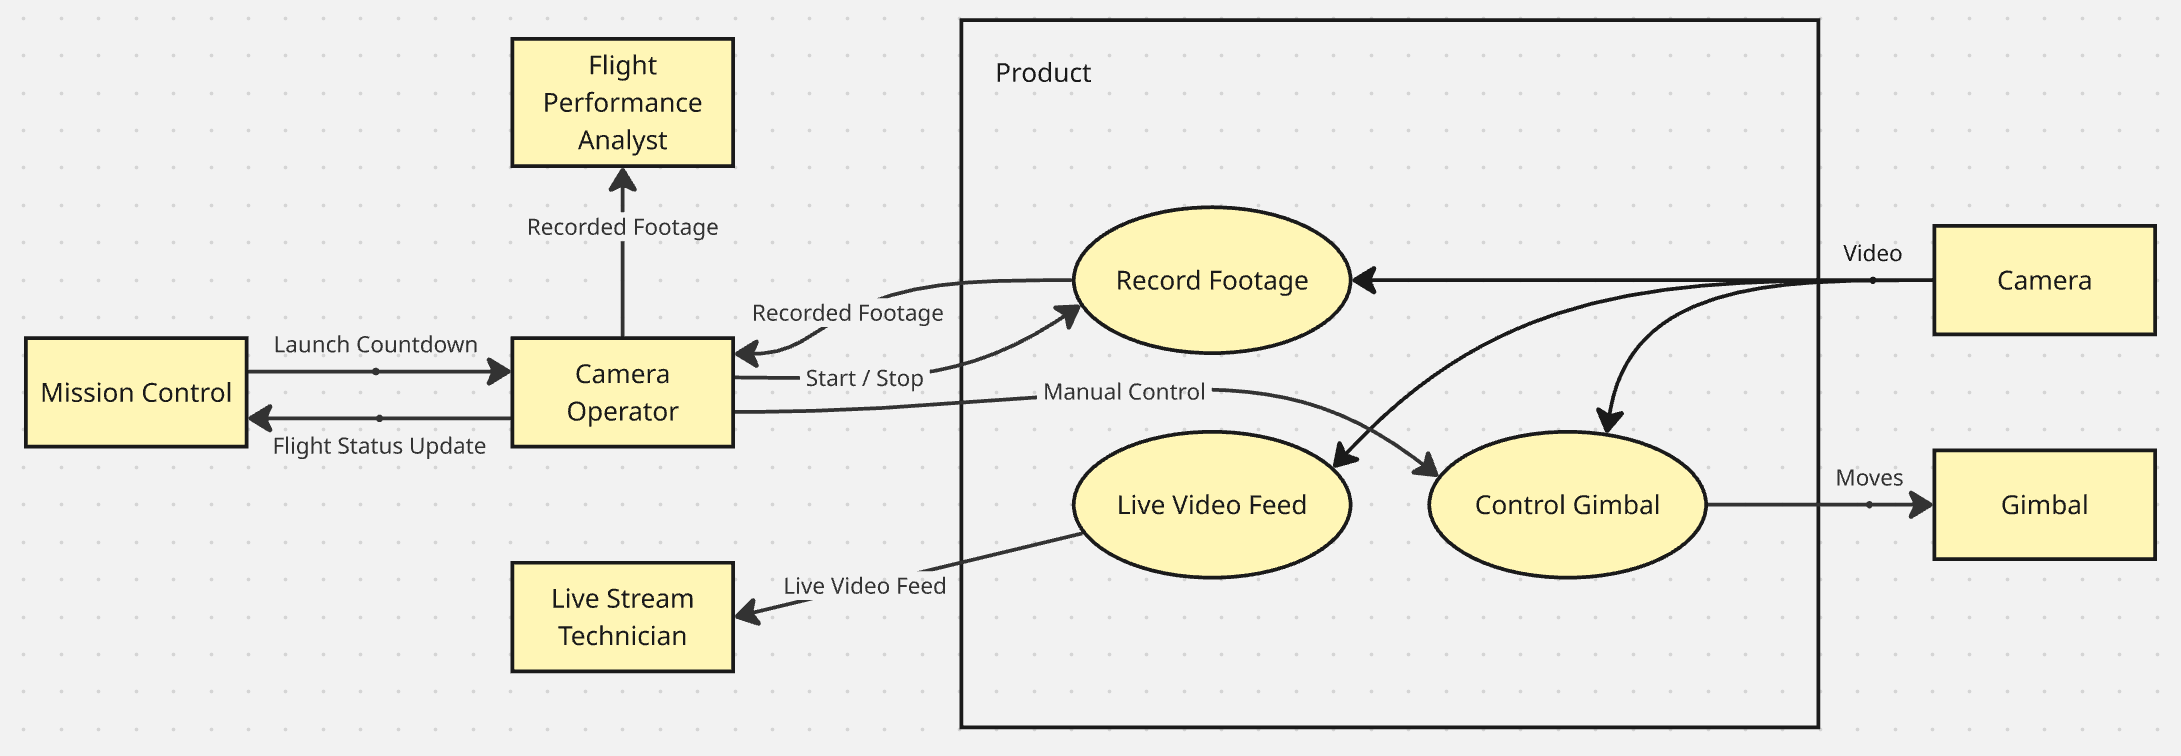
\includegraphics[width=\textwidth,height=\textheight,keepaspectratio]{../Images/product_boundary.png}
  \caption{Product Boundary}
  \label{img:product-boundary}
\end{figure}
\FloatBarrier

\subsection{Product Use Case Table}

The following \hyperref[tab:product-use-case-table]{Table 2} summarizes the
primary use cases of the system.

\begin{table}[H]
  \centering
  \setlength\extrarowheight{5mm}
  \begin{tabularx}{\textwidth}{p{0.4in}p{0.4in}p{1.25in}p{1in}X}
    \toprule \textbf{BUC No.}       & \textbf{PUC No.}        & \textbf{PUC Name}              &
    \textbf{Actors}                 & \textbf{Input / Output}                                    \\
    \midrule
    1                               & 1                       & Live video output              &
    Camera, Live Stream Technician
                                    &
    (in) Video feed from camera \newline
    (out) Live video output                                                                      \\
    2                               & 2.1                     & Point camera to rocket         &
    Camera Operator, Camera, Gimbal
                                    &
    (in) Manual gimbal adjustment commands from camera operator \newline
    (out) Movement commands to the gimbal                                                        \\
    2                               & 2.2                     & Start video recording          &
    Camera Operator, Camera
                                    &
    (in) Start video recording command \newline
    (out) Video recording started                                                                \\
    2                               & 2.3                     & Start tracking rocket          &
    Camera Operator, Camera, Gimbal
                                    &
    (in) Start tracking rocket command \newline
    (out) System in armed state                                                                  \\

    3                               & 3                       & Automated rocket tracking      &
    Camera, Gimbal                  &
    (in) Video feed from camera \newline
    (out) Movement commands to gimbal                                                            \\
    4                               & 4.1                     & Stop video recording           &
    Camera Operator, Camera         &
    (in) Stop video recording command \newline
    (out) Video recording stopped and saved                                                      \\
    4                               & 4.2                     & Stop tracking rocket           &
    Camera Operator, Camera, Gimbal &
    (in) Stop tracking rocket command \newline
    (out) Gimbal stops moving \newline
    (out) System in idle state                                                                   \\
    5                               & 5                       & View recorded footage and logs &
    Camera Operator                 &
    (in) request to download footage and logs \newline
    (out) Footage and logs downloaded                                                            \\

    \bottomrule
  \end{tabularx}
  \caption{Product Use Case Table}
  \label{tab:product-use-case-table}
\end{table}

\subsection{Individual Product Use Cases (PUC's)}

something something

~\\

\textbf{PUC 1: Live video output.}

\textbf{Actors:} Camera, Live Stream Technician.

\textbf{Preconditions:} The system is powered on and has finished initialization.

\textbf{Main Flow of Steps:}
\begin{enumerate}
  \item The camera operator connects the system to the live streaming equipments.
\end{enumerate}

\textbf{Outcome:} The live streaming equipments receive a video feed from the system.

~\\

\textbf{PUC 2.1: Point camera to rocket.}

\textbf{Actors:} Camera Operator, Camera, Gimbal.

\textbf{Preconditions:} The system is in idle state.

\textbf{Main Flow of Steps:}
\begin{enumerate}
  \item The camera operator monitors the camera preview on the UI.
  \item The camera operator selects the direction to rotate the gimbal on the UI.
  \item The system sends commands to the gimbal to rotate to the selected direction.
  \item The camera operator confirms the gimbal is rotating to the selected direction
        through the preview.
\end{enumerate}

\textbf{Outcome:} The gimbal is rotated to the selected direction.

~\\

\textbf{PUC 2.2: Start video recording.}

\textbf{Actors:} Camera Operator, Camera.

\textbf{Preconditions:} The system is powered on and has finished initialization; not currently recording.

\textbf{Main Flow of Steps:}
\begin{enumerate}
  \item The camera operator clicks the "Start Recording" button on the UI.
  \item The system starts to record the camera feed and additional logs (e.g. angle of
        the gimbal, temperature of the camera, etc.).
  \item The UI displays a recording indicator and the elapsed recording time.
\end{enumerate}

\textbf{Outcome:} Video recording starts and logs are written to storage.

~\\

\textbf{PUC 2.3: Start tracking rocket.}

\textbf{Actors:} Camera Operator, Camera, Gimbal.

\textbf{Preconditions:} System is in idle state.

\textbf{Main Flow of Steps:}
\begin{enumerate}
  \item The camera operator selects the "Arm" button on the UI.
  \item The system enters the armed state.
  \item The UI displays a "Armed" indicator.
\end{enumerate}

\textbf{Outcome:} The system enters the armed state and starts to look for rockets.

~\\

\textbf{PUC 3: Automated rocket tracking.}

\textbf{Actors:} Camera, Gimbal.

\textbf{Preconditions:} System is in armed state.

\textbf{Main Flow of Steps:}
\begin{enumerate}
  \item The system processes incoming frames to detect moving rockets.
  \item (Event) The system detects a moving rocket.
  \item The system enters the tracking state.
  \item The UI displays a "Tracking" indicator.
  \item The system sends movement commands to the gimbal to keep the rocket centered in
        the frame.
  \item If the rocket is lost, the system returns to idle state.
\end{enumerate}

\textbf{Outcome:} The gimbal follows the rocket and keeps it near the frame center until the rocket is lost.

~\\

\textbf{PUC 4.1: Stop video recording.}

\textbf{Actors:} Camera Operator, Camera.

\textbf{Preconditions:} The system is powered on and has finished initialization; currently recording.

\textbf{Main Flow of Steps:}
\begin{enumerate}
  \item The camera operator clicks the "Stop Recording" button on the UI.
  \item The system stops recording the camera feed and additional logs (e.g. angle of
        the gimbal, temperature of the camera, etc.).
  \item The system saves the video and logs to storage.
  \item The UI stops displaying the recording indicator.

\end{enumerate}

\textbf{Outcome:} Video recording stops.

~\\

\textbf{PUC 4.2: Stop tracking rocket.}

\textbf{Actors:} Camera Operator, Camera, Gimbal.

\textbf{Preconditions:} System is in armed or tracking state.

\textbf{Main Flow of Steps:}
\begin{enumerate}
  \item The camera operator clicks the "Stop Tracking" button on the UI.
  \item The system returns to idle state.
  \item The system stops sending movement commands to the gimbal.
  \item The UI displays a "Idle" indicator.
\end{enumerate}

\textbf{Outcome:} The system returns to idle state.

~\\

\textbf{PUC 5: View recorded footage and logs.}

\textbf{Actors:} Camera Operator.

\textbf{Preconditions:} The system is in idle state.

\textbf{Main Flow of Steps:}
\begin{enumerate}
  \item The camera operator opens the recordings page in the UI.
  \item The camera operator filters or selects the desired files by date/time.
  \item The camera operator downloads the files to their device.
\end{enumerate}

\textbf{Outcome:} The desired footage and logs are downloaded for offline viewing and analysis.

\subsection{System State Diagram}

The following is a state diagram of the system.

\FloatBarrier
\begin{figure}[h]
  \centering
  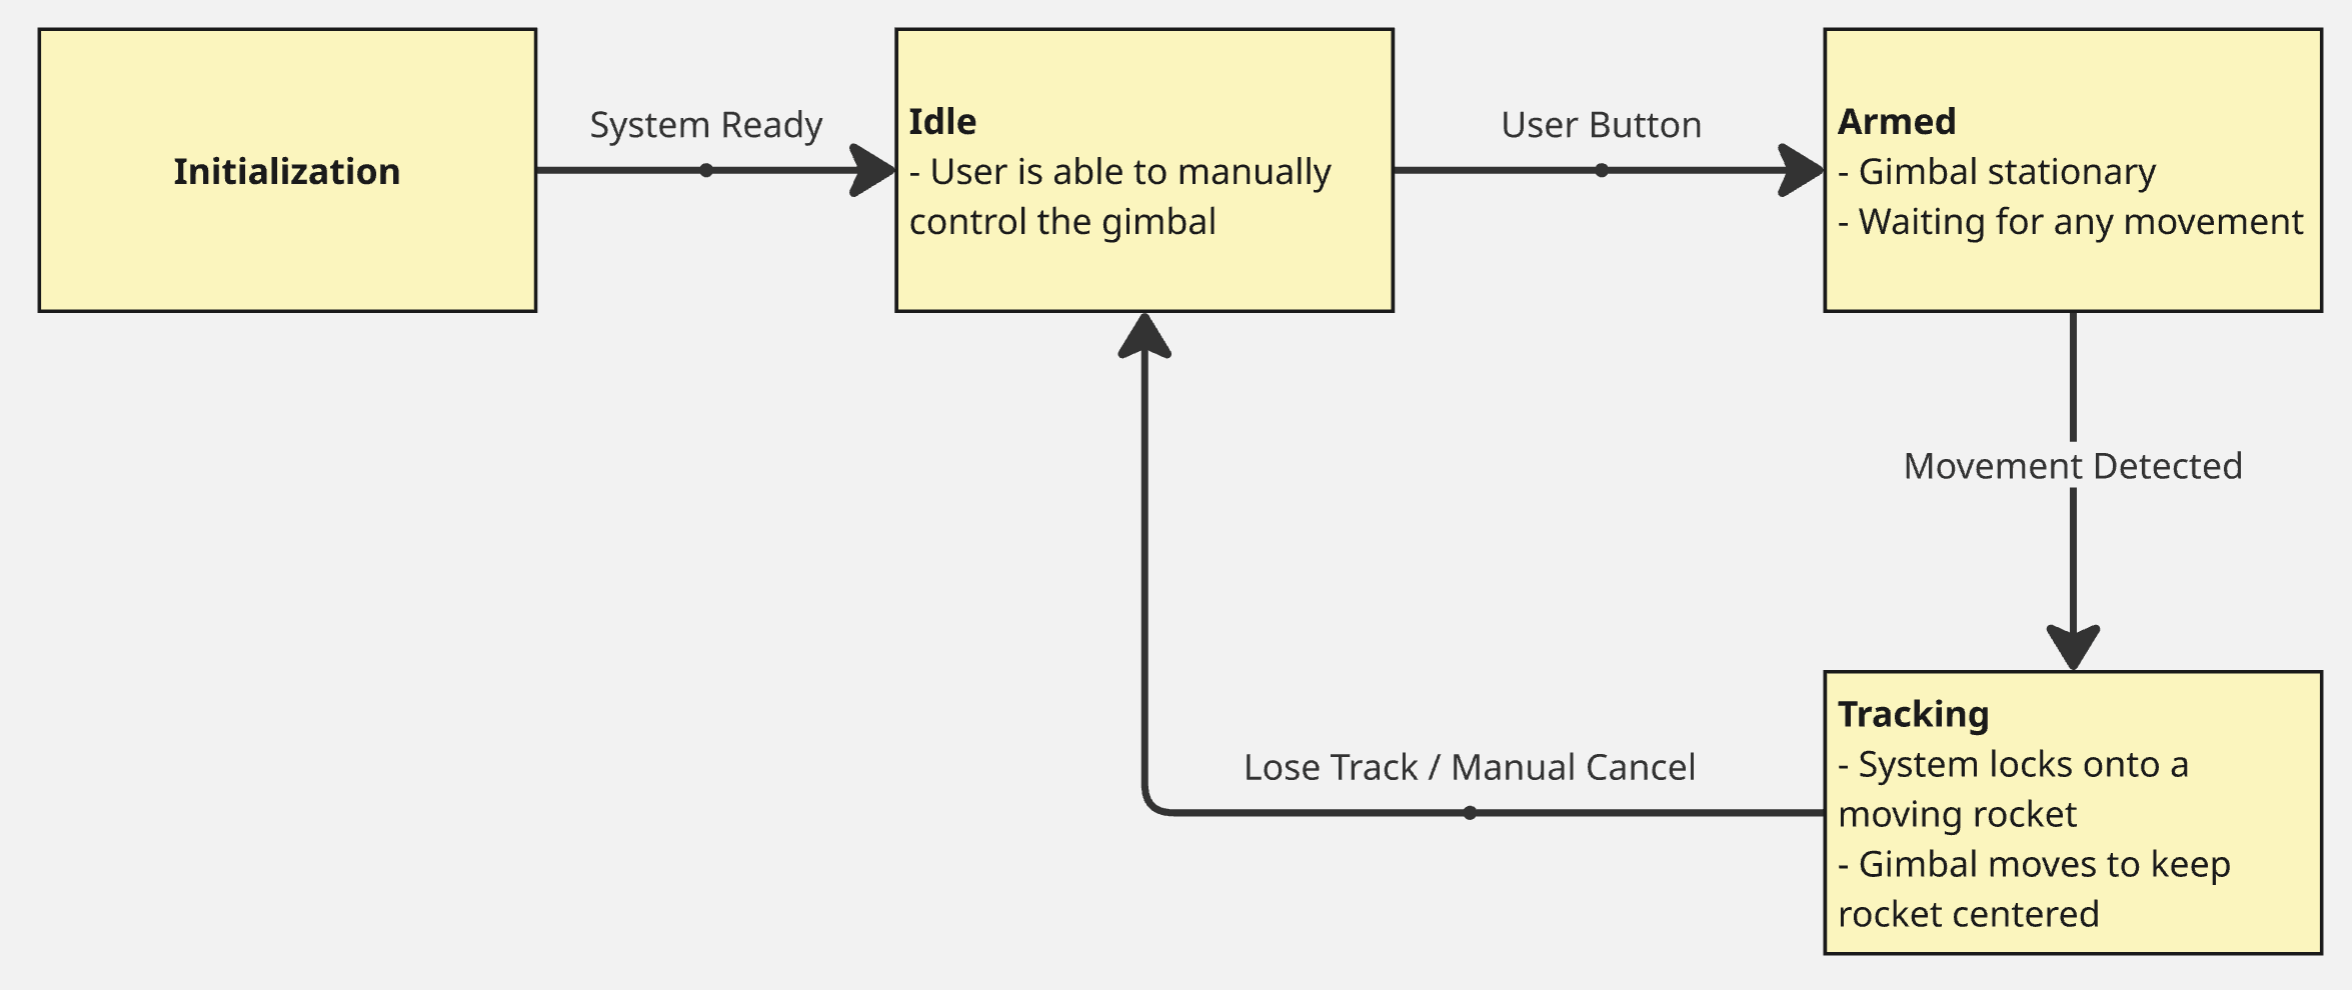
\includegraphics[width=\textwidth,height=\textheight,keepaspectratio]{../Images/state_diagram.png}
  \caption{System State Diagram}
  \label{img:state-diagram}
\end{figure}
\FloatBarrier

\section{Functional Requirements}
\subsection{Functional Requirements}

\begin{itemize}[leftmargin=*]

  \item[FR-1] \emph{The system must acquire live video stream from the connected
          camera.}\\[2mm]
        \textbf{Rationale:} Video acquisition is the first step of the vision-guided pipeline and enables all downstream processing.\\
        \textbf{Fit Criterion:} The system successfully captures frames at at least 1080p 60fps and passes them to the CV pipeline.\\
        \textbf{Source PUC:} PUC 1, PUC 3 \\
        \textbf{Priority:} High

  \item[FR-2] \emph{The system must send real-time movement commands to the connected
          gimbal.}\\[2mm]
        \textbf{Rationale:} Sending movement commands to gimbal is how the system controls the gimbal.\\
        \textbf{Fit Criterion:} Movement commands are sent to the gimbal at least once per video frame received.\\
        \textbf{Source PUC:} PUC2.1, PUC 3 \\
        \textbf{Priority:} High

  \item[FR-3] \emph{The system must detect moving rocket from the video stream in real
          time.}\\[2mm]
        \textbf{Rationale:} Real time rocket detection is the first step of the tracking process.\\
        \textbf{Fit Criterion:} The system can detect moving rockets from the video stream at 60fps.\\
        \textbf{Source PUC:} PUC 3 \\
        \textbf{Priority:} High

  \item[FR-4] \emph{If armed, the system must automatically enter the tracking state
          when a moving rocket is detected.}\\[2mm]
        \textbf{Rationale:} Entering the tracking state means the system is commanding the gimbal to keep the rocket centered in the frame.\\
        \textbf{Fit Criterion:} The system enters the tracking state when a moving rocket is detected.\\
        \textbf{Source PUC:} PUC 2.3, PUC 3 \\
        \textbf{Priority:} High

  \item[FR-5] \emph{If the system is in the tracking state and the rocket is lost, the
          system must automatically return to the idle state.}\\[2mm]
        \textbf{Rationale:} Automatically reverting to idle prevents unnecessary gimbal movement and prepares the system for future launches or manual intervention.\\
        \textbf{Fit Criterion:} Upon loss of the rocket target, the system transitions from tracking to idle state without manual input.\\
        \textbf{Source PUC:} PUC 3 \\
        \textbf{Priority:} High

  \item[FR-6] \emph{When in the idle state, the system must allow the user to manually
          control the gimbal.}\\[2mm]
        \textbf{Rationale:} Manual gimbal control is necessary for arming the camera to the launch pad before the rocket is launched.\\
        \textbf{Fit Criterion:} In idle mode, the user can issue manual pan/tilt commands that are reflected in real-time by the gimbal hardware.\\
        \textbf{Source PUC:} PUC 2.1 \\
        \textbf{Priority:} High

  \item[FR-7] \emph{When in the tracking state, and the rocket is not in view, the
          system must autonomously attempt re-acquisition, before declaring the rocket is
          lost.}\\[2mm]
        \textbf{Rationale:} Rocket may be temporarily obstructed; re-acquisition ensures robustness of the tracking process.\\
        \textbf{Fit Criterion:} The system waits for 2 seconds before declaring the rocket is lost.\\
        \textbf{Source PUC:} PUC 3 \\
        \textbf{Priority:} Medium

  \item[FR-8] \emph{When in the tracking state, the system must autonomously keep the
          rocket within the frame.}\\[2mm]
        \textbf{Rationale:} Accurate rocket tracking is the core function of the system.\\
        \textbf{Fit Criterion:} Rocket remains within visible in the frame.\\
        \textbf{Source PUC:} PUC 3 \\
        \textbf{Priority:} High

  \item[FR-9] \emph{The system must begin outputting video through HDMI as soon as it
          is initialized.}\\[2mm]
        \textbf{Rationale:} Immediate HDMI output ensures that event video is available to stakeholders from the earliest possible moment.\\
        \textbf{Fit Criterion:} Upon system initialization, an HDMI-connected display immediately receives a live video signal from the camera without requiring additional user action.\\
        \textbf{Source PUC:} PUC 1 \\
        \textbf{Priority:} High

  \item[FR-10] \emph{The HDMI video output must have a text overlay that displays the
          current gimbal tilt and pan angle.}\\[2mm]
        \textbf{Rationale:} Overlaying the gimbal angles on the video stream provides immediate feedback to operators and analysts and aids in diagnostics and post-flight analysis.\\
        \textbf{Fit Criterion:} The HDMI output includes a text label showing current tilt and pan angles, updating once per video frame.\\
        \textbf{Source PUC:} PUC 1 \\
        \textbf{Priority:} Medium

  \item[FR-11] \emph{The system must display runtime information including system state
          and camera preview to the user.}\\[2mm]
        \textbf{Rationale:} Seeing the system status and camera preview is necessary for the user to control the system.\\
        \textbf{Fit Criterion:} The interface updates system status and preview in real time with at least 15fps.\\
        \textbf{Source PUC:} PUC 2.1 \\
        \textbf{Priority:} High

  \item[FR-12] \emph{The system must only enter armed mode when explicitly instructed
          by the user.}\\[2mm]
        \textbf{Rationale:} Prevents accidental or unintended transitions to armed state, ensuring safe and predictable operation for all users.\\
        \textbf{Fit Criterion:} The system transitions from idle to armed mode only in response to a clear, user-initiated command, and never automatically or implicitly.\\
        \textbf{Source PUC:} PUC 2.3 \\
        \textbf{Priority:} High

  \item[FR-13] \emph{The system must allow users to record video and logs associated
          with the video for later review.}\\[2mm]
        \textbf{Rationale:} Recording supports debugging, validation, and demonstration.\\
        \textbf{Fit Criterion:} Users can start and stop recording from the UI.\\
        \textbf{Source PUC:} PUC 2.2, PUC 4.1 \\
        \textbf{Priority:} High

  \item[FR-14] \emph{The system must provide management functionalities for recorded
          videos and logs (list, delete, download).}\\[2mm]
        \textbf{Rationale:} Reviewing and managing captured sessions supports performance analysis and documentation.\\
        \textbf{Fit Criterion:} Users can view the list of recorded videos and logs, and perform delete/download actions.\\
        \textbf{Source PUC:} PUC 5 \\
        \textbf{Priority:} High

\end{itemize}
\section{Look and Feel Requirements}
\subsection{Appearance Requirements}
\begin{itemize}[leftmargin=*]
  \item[AR-1] \emph{The user interface shall be designed for higher readability in
          outdoor environments}\\[2mm]
        \textbf{Rationale:} The system is going to be used in outdoor environments\\
        \textbf{Fit Criterion:} Test users report no issues with readability in outdoor environments

  \item[AR-2] \emph{All UI elements required for tracking operation shall be visible in
          one page without scrolling on a 1080p display.}\\[2mm]
        \textbf{Rationale:} Operators need immediate awareness of system
        status under high-pressure launch operations.\\
        \textbf{Fit Criterion:} On a 1920x1080 monitor, all UI elements required for tracking operation are visible without scrolling
\end{itemize}

\subsection{Style Requirements}
\begin{itemize}[leftmargin=*]
  \item[SR-1] \emph{The user interface shall appear professional and reliable}\\[2mm]
        \textbf{Rationale:} The system is controlling a physical gimbal and it is important to gain the trust of the users.\\
        \textbf{Fit Criterion:} More than 80\% of Test users report the system appears professional and reliable
\end{itemize}

\section{Usability and Humanity Requirements}
\subsection{Ease of Use Requirements}
\begin{itemize}[leftmargin=*]
  \item[EZ-1] \emph{Units in the user interface shall be consistent}\\[2mm]
        \textbf{Rationale:} Consistency reduces operator error during high-pressure launch operations.\\
        \textbf{Fit Criterion:} A style audit of UI readouts finds no unit inconsistencies.

  \item[EZ-2] \emph{All user interface interactions shall provide immediate feedback to
          the user.}\\[2mm]
        \textbf{Rationale:} Immediate feedback reassures users that the system has registered their actions and helps prevent confusion or repeated actions during critical operations.\\
        \textbf{Fit Criterion:} For all UI actions, a visible confirmation appears within 0.2 seconds of user input in usability tests.

  \item[EZ-3] \emph{The system shall rely on visual indicators for system status and
          alerts.}\\[2mm]
        \textbf{Rationale:} The work environment may be noisy or require hearing protection, so visual cues ensure users do not miss important updates or warnings.\\
        \textbf{Fit Criterion:} All status and alerts are presented visually in the UI.
  \item[EZ-4] \emph{The product shall help the user to avoid making mistakes.}\\[2mm]
        \textbf{Rationale:} Because the system is connected to a physical gimbal, a user error might cause significant damage.\\
        \textbf{Fit Criterion:} Every potentially dangerous command presents a confirmation prompt that must be acknowledged before proceeding.
\end{itemize}

\subsection{Personalization and Internationalization Requirements}
\begin{itemize}[leftmargin=*]
  \item[PI-1] \emph{The user interface shall support both metric and imperial units}\\[2mm]
        \textbf{Rationale:} Allowing the user to pick the unit system with which they are most familiar helps reduce user mistakes. \\
        \textbf{Fit Criterion:} Unit preferences can be selected and applied to the UI.
  \item[PI-2] \emph{The user interface shall support both English and French
          languages}\\[2mm]
        \textbf{Rationale:} Bilingual support meets accessibility and inclusiveness standards for Canadian stakeholders and allows operation by users from different linguistic backgrounds.\\
        \textbf{Fit Criterion:} Users can select either English or French, and all UI text is presented in the chosen language.
\end{itemize}

\subsection{Learning Requirements}
\begin{itemize}[leftmargin=*]
  \item[LR-1] \emph{The system shall be easy to learn for users with a reasonable level
          of technological familiarity, provided they have access to the instruction
          manual.}\\[2mm]
        \textbf{Rationale:} Reducing the learning curve for technically literate users allows for faster and safer adoption, especially in time-pressured launch scenarios.\\
        \textbf{Fit Criterion:} In usability tests, new users who have read the manual are able to successfully perform all product use cases within 20 minutes without external assistance.

\end{itemize}

\subsection{Understandability and Politeness Requirements}
\begin{itemize}[leftmargin=*]
  \item[UPR-1] \emph{The system shall use symbols and words that are naturally
          understandable by the user community.}\\[2mm]
        \textbf{Rationale:} Using familiar terminology and icons reduces cognitive load and misinterpretation, especially during high-pressure tasks.\\
        \textbf{Fit Criterion:} User testing confirms that 90\% of surveyed users recognize and correctly interpret all UI symbols and labels without additional explanation.

  \item[UPR-2] \emph{The system should only display information required for normal use
          cases on the main page (i.e., hide debug information).}\\[2mm]
        \textbf{Rationale:} Restricting the main interface to essential information keeps the UI clear and reduces distraction or confusion for non-technical users.\\
        \textbf{Fit Criterion:} Reviews confirm that only operational and safety-relevant details are visible to end users during normal workflows; diagnostic/debug fields require an explicit action to reveal.

  \item[UPR-3] \emph{All confirmation dialogs should explain why an action could
          potentially be dangerous.}\\[2mm]
        \textbf{Rationale:} Providing context in confirmation dialogs educates users, prevents accidental execution of risky commands, and reinforces safe operational habits when interacting with hardware.\\
        \textbf{Fit Criterion:} All confirmation dialogs for safety-critical actions include a clear, specific explanation of risk, as verified by interface inspection.
\end{itemize}

\subsection{Accessibility Requirements}
\begin{itemize}[leftmargin=*]
  \item[AR-1] \emph{Status indicators shall remain distinguishable under common
          color-vision deficiencies.}\\[2mm]
        \textbf{Rationale:} Ensures legibility for diverse users and conditions.\\
        \textbf{Fit Criterion:} UI passes color-vision simulations.
\end{itemize}

\section{Performance Requirements}
\subsection{Speed and Latency Requirements}
\begin{itemize}[leftmargin=*]
  \item[SLR-1] \emph{camera-to-gimbal latency shall be low enough to enable continuous
          rocket tracking.}\\[2mm]
        \textbf{Rationale:} If the latency is too high, the gimbal will not ba able to keep up with the rocket\\
        \textbf{Fit Criterion:} Field tests confirm the latency is low enough to enable continuous rocket tracking.

  \item[SLR-2] \emph{The system shall be able to handle 1080p 60fps camera feed}\\[2mm]
        \textbf{Rationale:} The camera feed is the input to the system\\
        \textbf{Fit Criterion:} The system is able to handle 1080p 60fps camera feed.

  \item[SLR-3] \emph{The system shall be able to output 1080p 60fps video via HDMI}\\[2mm]
        \textbf{Rationale:} The HDMI output is the output of the system\\
        \textbf{Fit Criterion:} The system is able to output 1080p 60fps video via HDMI.
\end{itemize}

\subsection{Safety-Critical Requirements}
\begin{itemize}[leftmargin=*]
  \item[SCR-1] \emph{The system must allow the user to manually exit armed or tracking
          mode, transitioning the system to idle mode.}\\[2mm]
        \textbf{Rationale:} Manual override is necessary to ensure safety, provide user control in unexpected circumstances, and to prepare the system for the next operation.\\
        \textbf{Fit Criterion:} When the user issues an exit command during armed or tracking mode, the system transitions to idle mode within 0.5 second and ceases any automated gimbal movement.\\
        \textbf{Source PUC:} PUC 4.2 \\
        \textbf{Priority:} High
\end{itemize}

\subsection{Precision or Accuracy Requirements}
\begin{itemize}[leftmargin=*]
  \item[PAR-1] \emph{In the recorded footage and the live stream, the rocket shall be
          centered in the frame}\\[2mm]
        \textbf{Rationale:} Stable footage is important for the analysis of the flight\\
        \textbf{Fit Criterion:} The user is satisfied with the stability of the footage.
\end{itemize}

\subsection{Robustness or Fault-Tolerance Requirements}
\begin{itemize}[leftmargin=*]
  \item[RFR-1] \emph{The system shall report all errors to the user interface for
          timely notification and resolution.}\\[2mm]
        \textbf{Rationale:} Immediate visibility of errors ensures users can respond quickly, improving system safety and reliability.\\
        \textbf{Fit Criterion:} Any error condition, including hardware faults, communication losses, and software exceptions, generates a visible and descriptive message on the user interface as verified during failure injection testing.
  \item[RFR-2] \emph{The system shall immediately stop all automated operations and
          enter a safe state if any unrecoverable error occurs.}\\[2mm]
        \textbf{Rationale:} Rapid cessation of activity prevents damage to equipment and ensures user safety when continued operation is unsafe.\\
        \textbf{Fit Criterion:} Simulated unrecoverable errors (such as critical hardware failures or fatal software exceptions) cause the system to halt actuation and notify the user interface within 1 second.
\end{itemize}

\subsection{Capacity Requirements}
\begin{itemize}[leftmargin=*]
  \item[CR-1] \emph{The system must provide sufficient storage capacity to record at
          least 100 launches.}\\[2mm]
        \textbf{Rationale:} Ensures adequate capacity for a full series of events without requiring immediate offloading, supporting typical event schedules and operational continuity.\\
        \textbf{Fit Criterion:} System verifies available storage prior to use; test runs confirm that at least 100 launches are recorded and preserved without storage exhaustion.
\end{itemize}

\subsection{Scalability or Extensibility Requirements}

None.

\subsection{Longevity Requirements}

None.

\section{Operational and Environmental Requirements}
\subsection{Expected Physical Environment}
- noisy
- bright
- wide temperature range
\begin{itemize}[leftmargin=*]
  \item[EPE-1] \emph{The system shall operate normally—without overheating, system
          instability, or degraded performance—within the expected deployment
          environments.}\\[2mm]
        \textbf{Rationale:} Outdoor launch sites can present challenging ambient conditions; hardware and software must tolerate these environments reliably.\\
        \textbf{Fit Criterion:} During field trials at representative sites, the system remains stable and fully functional through a typical launch day, with no evidence of thermal shutdown or operating errors due to the environment.
\end{itemize}

\subsection{Wider Environment Requirements}

None.

\subsection{Requirements for Interfacing with Adjacent Systems}

- must use HDMI
- must provide a flexible interface for gimbal hardware

\begin{itemize}[leftmargin=*]
  \item[OER-INT-1] \emph{Provide an HDMI program feed and an IP stream compatible with
          common switchers/encoders; remote control range shall be $\geq$ 100\,m.}\\
        \textbf{Rationale:} Integrates with broadcast rigs and supports distant safe
        operation.\\ \textbf{Fit Criterion:} Verified ingest into OBS/capture cards;
        stable remote control over a measured 100\,m link.
\end{itemize}

\subsection{Productization Requirements}

None.

\subsection{Release Requirements}

- one release will be made by the end of the project
\begin{itemize}[leftmargin=*]
  \item[OER-REL-1] \emph{Each public release shall include a parameter sheet and links
          to system, network, and support documentation.}\\ \textbf{Rationale:} Speeds
        onboarding of new crew and stakeholders.\\ \textbf{Fit Criterion:} Release
        bundle contains the parameter sheet and referenced chapters.
\end{itemize}

\section{Maintainability and Support Requirements}

Not applicable, no features or changes are expected to be made after the
project is completed.

\subsection{Supportability Requirements}

Not applicable.

\subsection{Adaptability Requirements}

Not applicable, we are free to pick any hardware platform.

\section{Security Requirements}
\subsection{Access Requirements}

Not applicable, we assume that the system will not be connected to the public
internet, and only physically accessible by authorized personnel.

\subsection{Integrity Requirements}
\begin{itemize}[leftmargin=*]
  \item[SEC-IT-1] \emph{The system shall validate all user inputs to prevent invalid
          commands from being sent to the gimbal.}\\ \textbf{Rationale:} Prevents
        accidental or malicious input errors that could result in unsafe or unintended
        gimbal motion.\\ \textbf{Fit Criterion:} All gimbal control inputs from the
        user interface are checked for validity and range prior to execution; test
        cases confirm that malformed or out-of-range commands are rejected and not
        transmitted to the gimbal.
\end{itemize}

\subsection{Privacy Requirements}

None.

\subsection{Audit Requirements}
\begin{itemize}[leftmargin=*]
  \item[SEC-AU-1] \emph{The system shall log all operations performed by the user,
          recording each action with a timestamp.}\\ \textbf{Rationale:} Comprehensive
        logging increases traceability, supports troubleshooting, and ensures
        accountability by maintaining an accurate record of user activity.\\
        \textbf{Fit Criterion:} For every operation executed via the user interface,
        the system appends an entry to the log including the nature of the operation,
        the user (if applicable), and an accurate timestamp; audit tests confirm no
        user action proceeds unlogged.
\end{itemize}

\subsection{Immunity Requirements}

Not applicable, we assume that the system will not be connected to the public
internet, and only physically accessible by authorized personnel.

\section{Cultural Requirements}
\begin{itemize}[leftmargin=*]
  \item[CUL-1] \emph{The system must avoid using colours or symbols that could be
          culturally sensitive or offensive.}\\ \textbf{Rationale:} Ensuring cultural
        sensitivity in design helps avoid alienating or offending users from diverse
        backgrounds, which is critical for global acceptance and usability.\\
        \textbf{Fit Criterion:} Conduct a cultural review to ensure that all icons and
        colours used in the tool are neutral and universally acceptable.
  \item[CUL-2] \emph{The system must not include content that could be considered
          culturally insensitive.}\\ \textbf{Rationale:} Avoiding culturally insensitive
        content ensures that the tool is respectful and inclusive, fostering a positive
        user experience across different cultures.\\ \textbf{Fit Criterion:} A cultural
        sensitivity review is conducted to ensure all content is appropriate for a
        global audience.
\end{itemize}

\section{Compliance Requirements}
\subsection{Legal Requirements}
\begin{itemize}[leftmargin=*]
  \item[CMP-LG-1] \emph{The system must respect user privacy by avoiding the collection
          of any personal or identifiable data.}\\ \textbf{Rationale:} Ensuring privacy
        builds user trust and minimizes risks associated with handling sensitive
        information, even when specific privacy laws are not targeted.\\ \textbf{Fit
          Criterion:} The system avoids collecting or storing personal user data,
        including information about user activities and profiles, and operates entirely
        within the user's local environment.
\end{itemize}

\subsection{Standards Compliance Requirements}

None.

% xxxxxxxxxxxxxxxxxxxxxxxxxxxxxxxxxx 18 xxxxxxxxxxxxxxxxxxxxxxxxxxxxxxxxxxxxxxxxxxxxx
\section{Open Issues}
\label{sec:open-issues}

This section lists open questions that could affect RoCam’s design, operation, and deployment. Each issue states why it matters, how we will close it with a test, who owns it, a due date aligned to the POC window (Nov. 17–28, 2025), and trace notes for bi-directional traceability. Acronyms are defined on first use: frames per second (FPS); field of view (FOV).

\subsection*{OI-01 — End-to-end rocket tracking feasibility}
\textbf{Summary:} Can we reliably lock, keep centered, and reacquire a small, fast rocket?\\
\textbf{Why it matters:} This is RoCam’s core value.\\
\textbf{Closure test:} Field tests show a median center error at most 20 pixels and reacquisition in at most 1.0 seconds across at least 5 launches.\\
\textbf{Owner:} CV Lead; Motion Control Lead \quad \textbf{Due:} 2025-11-20\\
\textbf{Trace:} FR-Tracking-Loop, FR-Reacquire; POC Steps 2–4; V\&V Plan.

\subsection*{OI-02 — Jetson pipeline performance (capture to inference to control)}
\textbf{Summary:} Validate FPS and latency on target hardware.\\
\textbf{Why it matters:} Low latency enables smooth gimbal motion.\\
\textbf{Closure test:} End-to-end latency at most 120 ms while sustaining at least 30 FPS; report median and 95th percentile.\\
\textbf{Owner:} CV Lead \quad \textbf{Due:} 2025-11-10\\
\textbf{Trace:} NFR-Performance; FR-Tracking-Loop; Expected Technology (CV).

\subsection*{OI-03 — Gimbal slew and STM32 control stability}
\textbf{Summary:} Check max pan/tilt speeds and controller stability under rocket rates.\\
\textbf{Why it matters:} Hardware must keep up without oscillation.\\
\textbf{Closure test:} Step and ramp tests show no instability; max slew at least 180 deg/s; overshoot at most 5 percent.\\
\textbf{Owner:} Motion Control Lead \quad \textbf{Due:} 2025-11-10\\
\textbf{Trace:} FR-Gimbal-Control; NFR-Safety; POC Step 4.

\subsection*{OI-04 — Occlusion, smoke, glare and backlight handling}
\textbf{Summary:} Robust tracking in difficult visuals; automatic reacquire.\\
\textbf{Why it matters:} Launches include plume/smoke and changing light.\\
\textbf{Closure test:} Scripted tests with occluders and backlight achieve at least 90 percent successful reacquisition within 1.0 seconds.\\
\textbf{Owner:} CV Lead; QA \quad \textbf{Due:} 2025-11-15\\
\textbf{Trace:} FR-Reacquire, FR-Tracking-Loop; V\&V scenarios.

\subsection*{OI-05 — Web preview latency and control responsiveness}
\textbf{Summary:} Measure browser preview delay and UI command round-trip on field network.\\
\textbf{Why it matters:} Operator needs near real-time feedback.\\
\textbf{Closure test:} Preview 95th percentile latency at most 300 ms; command round-trip at most 150 ms on site Wi-Fi or hotspot.\\
\textbf{Owner:} Web Lead \quad \textbf{Due:} 2025-11-15\\
\textbf{Trace:} FR-Web-Preview, FR-Remote-Control; NFR-Usability.

\subsection*{OI-06 — Target size versus lens, FOV, and stand-off distance}
\textbf{Summary:} Ensure rocket has enough pixels for detection and tracking.\\
\textbf{Why it matters:} Too small a target breaks detection.\\
\textbf{Closure test:} Optics sizing shows at least 30 pixels of target height at the minimum distance; confirmed in ground tests.\\
\textbf{Owner:} CV Lead; HW Lead \quad \textbf{Due:} 2025-11-05\\
\textbf{Trace:} FR-Image-Acquisition, FR-Detect-Motion; POC Step 1.

\subsection*{OI-07 — Recording and archival (format, bitrate, storage, retrieval)}
\textbf{Summary:} Decide how to record video and make it available.\\
\textbf{Why it matters:} Needed for demos, analysis, and V\&V evidence.\\
\textbf{Closure test:} Recording at 1920x1080 and 30 FPS with storage rotation; operator can download footage via the web UI.\\
\textbf{Owner:} Web Lead; CV Lead \quad \textbf{Due:} 2025-11-18\\
\textbf{Trace:} FR-Recording, FR-Web-Download; NFR-Storage.

\subsection*{OI-08 — Site networking and power plan}
\textbf{Summary:} Confirm bandwidth and stable power at launch site(s).\\
\textbf{Why it matters:} Unreliable links or power will break the demo.\\
\textbf{Closure test:} Site checklist complete; backup link tested; UPS or batteries sized for at least 30 minutes of runtime.\\
\textbf{Owner:} Field Ops; HW Lead \quad \textbf{Due:} 2025-11-12\\
\textbf{Trace:} NFR-Reliability; Ops-Readiness; POC logistics.

\subsection*{OI-09 — Safety and abort in the web UI}
\textbf{Summary:} Define operator authority, safe states, and emergency stop flow.\\
\textbf{Why it matters:} Must halt motion safely on faults or command.\\
\textbf{Closure test:} From any state, emergency stop reaches a safe state within at most 200 ms; procedure documented and tested.\\
\textbf{Owner:} Motion Control Lead; Web Lead; QA \quad \textbf{Due:} 2025-11-16\\
\textbf{Trace:} NFR-Safety; FR-Gimbal-Control; Hazard Analysis.

\subsection*{OI-10 — Integration interfaces (CV, STM32, Web)}
\textbf{Summary:} Freeze message schemas and timing expectations.\\
\textbf{Why it matters:} Reduces late integration risk.\\
\textbf{Closure test:} Versioned API documents published; bench integration test passes three consecutive runs without timeouts.\\
\textbf{Owner:} Subproject Leads; QA facilitator \quad \textbf{Due:} 2025-11-08\\
\textbf{Trace:} Cross-cutting FRs; POC risk “Integration”.

\subsection*{OI-11 — Environmental readiness (wind, lighting, Jetson thermals)}
\textbf{Summary:} Validate operation under expected weather and heat.\\
\textbf{Why it matters:} Outdoor launches vary.\\
\textbf{Closure test:} Test matrix executed; Jetson temperatures at or below 80 C with no throttling during a 30 minute run.\\
\textbf{Owner:} Platform Eng.; Field Ops \quad \textbf{Due:} 2025-11-14\\
\textbf{Trace:} NFR-Performance; NFR-Reliability; Ops-Readiness.

\subsection*{OI-12 — Operator workflow and usability}
\textbf{Summary:} Make target pick, mode switch, and errors simple and clear.\\
\textbf{Why it matters:} Reduces operator mistakes during demos.\\
\textbf{Closure test:} Five-user hallway test: at least four of five complete tasks unaided; System Usability Scale score at least 75.\\
\textbf{Owner:} Web Lead; QA \quad \textbf{Due:} 2025-11-18\\
\textbf{Trace:} NFR-Usability; FR-Target-Selection; Web App.

\subsection*{OI-13 — Install and update (Jetson/STM32) and rollback}
\textbf{Summary:} Define install steps, versioning, and rollback.\\
\textbf{Why it matters:} The rubric requires installability; reliable updates reduce field risk.\\
\textbf{Closure test:} Cold install in at most 10 minutes; one-command update and rollback verified on a clean device.\\
\textbf{Owner:} Platform Eng. \quad \textbf{Due:} 2025-11-12\\
\textbf{Trace:} NFR-Installability; CI/CD; Expected Technology.

\subsection*{OI-14 — Data retention and privacy}
\textbf{Summary:} Set retention period and access rules for footage and logs.\\
\textbf{Why it matters:} Manages storage and sharing expectations.\\
\textbf{Closure test:} Policy documented; maximum retention of 30 days enforced automatically; access control tested.\\
\textbf{Owner:} PM; Web Lead \quad \textbf{Due:} 2025-11-18\\
\textbf{Trace:} NFR-Security and Privacy; FR-Recording and Logs.



\section{Off-the-Shelf Solutions}
% xxxxxxxxxxxxxxxxxxxxxxxxxxxxxxxxxx 19.1 xxxxxxxxxxxxxxxxxxxxxxxxxxxxxxxxxxxxxxxxxxxxx
\subsection{Ready-Made Products}
\label{sec:ready-made-products}

\textbf{Conclusion:} No off-the-shelf product reliably tracks a small, fast rocket end-to-end.

\textbf{Surveyed:} consumer/prosumer camera trackers; sports/wildlife auto-tracking; industrial/defense PTZ trackers.

\textbf{Criteria:} acquire/re-acquire small target; keep centered at high speed; low latency; operator control/safety; integration (camera, gimbal, web); logging.

\textbf{Findings (Gaps):}
\begin{itemize}[noitemsep,topsep=2pt]
  \item Target too small / motion too fast.
  \item Weak occlusion/smoke re-acquire.
  \item Latency not specified or too high.
  \item Closed stacks; poor API/integration.
  \item Limited safety controls and logs.
\end{itemize}

\textbf{Decision:} Build custom solution (meets performance, safety, integration needs).

\textbf{Revisit:} Reassess if a vendor demonstrates low-latency, small-target tracking with open APIs.


% xxxxxxxxxxxxxxxxxxxxxxxxxxxxxxxxxx 19.2 xxxxxxxxxxxxxxxxxxxxxxxxxxxxxxxxxxxxxxxxxxxxx
\subsection{Reusable Components}
\label{sec:reusable-components}

Below are the key open-source components RoCam will reuse. For each, we explain what it does, where it comes from, and why it is a good fit. Each choice is simple to verify with clear measurements and has low integration risk.

\paragraph{OpenCV (Python).}
OpenCV will handle camera capture, reading and writing frames, basic image operations, and drawing overlays for the live preview. It is open source under a BSD license and is widely used on NVIDIA Jetson devices. We can verify it easily by measuring frames per second and end-to-end latency during live capture and by checking that overlays appear correctly on the preview.

\paragraph{Ultralytics YOLO.}
Ultralytics YOLO will provide object detection to find the rocket and keep the track initialized. It is open source and has models that balance accuracy and speed on edge hardware. We will test it on sample launch videos and measure precision, recall, and inference time to confirm it meets our target speed and detection quality.

\paragraph{PyTorch and TorchVision.}
PyTorch and TorchVision will run the detection models, perform preprocessing, and support simple experiments such as quantization. They are open source with a permissive license and work well with CUDA on the Jetson platform. We will verify them by timing the full pipeline on our device and confirming that model outputs are correct on a small labeled clip set.

\paragraph{Optical Flow (OpenCV).}
We will use OpenCV’s optical flow to add motion cues that help with small or fast targets and to support re-acquisition if the detector misses a frame. This component is open source and lightweight. We will compare re-acquisition time and tracking continuity with and without optical flow on the same sequences to confirm the benefit.

\paragraph{NVIDIA JetPack SDK.}
JetPack provides CUDA, cuDNN, multimedia libraries, and device drivers required for the Jetson. It is a free vendor SDK. Using JetPack reduces custom integration work and enables hardware acceleration. We will verify correct setup by running a small GPU self-test, confirming camera capture works, and measuring that model inference uses the GPU.

\paragraph{STM32 with \texttt{embassy-rs} (Rust).}
The STM32 microcontroller and the \texttt{embassy-rs} async runtime will run the real-time gimbal control loop, including timers, GPIO, and serial links. These crates are open source and build on \texttt{embedded-hal}. We will verify control quality using simple step and ramp tests, checking for stable response, acceptable overshoot, and maximum slew rate.

\paragraph{Flask (Backend).}
Flask will serve a small HTTP and WebSocket API for control, status, and video preview endpoints. It is open source under a BSD license, easy to containerize, and simple to read and test. We will verify the API with unit tests for each route and with a basic integration test that starts, arms, begins tracking, and stops through the web interface.

\paragraph{React (Frontend).}
React will power the operator web interface for connect, arm, start and stop tracking, target selection, and status. It is open source under an MIT license and has a strong ecosystem. We will verify usability with short hallway tests, looking at task completion, time to perform key actions, and a simple usability score.

\paragraph{GStreamer or FFmpeg.}
We will use GStreamer or FFmpeg for video encoding, streaming, and recording. Both are open source and proven on Jetson. We will verify preview and recording by measuring median and tail preview latency, checking for dropped frames, and confirming that recorded files play back at the expected resolution and frame rate.

\paragraph{Docker.}
Docker will be used to containerize the computer vision and backend services to ensure repeatable builds and installs. It is open source (Moby/Apache 2.0). We will verify installability by performing a clean install on a fresh device, running one command to start services, and testing a simple rollback of a container image.

\paragraph{GitHub Actions.}
GitHub Actions will provide continuous integration for builds, unit tests, style checks, and container images. It has a free tier for public use. We will verify it by enforcing that each pull request runs linting and tests, produces a build artifact, and fails if coverage or style gates are not met.

\medskip
\noindent\textbf{Verification approach for all components.}
For every component above we will record the version and license, define one or more clear checks (for example frames per second, latency, precision and recall, controller step response, and web task success), and store the results with links back to the requirement they support. This keeps our reuse choices measurable and traceable.




% xxxxxxxxxxxxxxxxxxxxxxxxxxxxxxxxxx  xxxxxxxxxxxxxxxxxxxxxxxxxxxxxxxxxxxxxxxxxxxxx

\subsection{Products That Can Be Copied}
\label{sec:products-that-can-be-copied}

RoCam can adopt proven interface and workflow patterns from adjacent products to reduce risk and speed delivery. The most relevant sources are:
\textit{surveillance PTZ camera consoles} (clear live preview, crosshair, presets),
\textit{drone ground control stations} (arm/disarm, mode switching, prominent safety actions),
\textit{IP/action camera apps} (record/stop, timers, storage indicators, simple download),
and \textit{low-latency web viewers} (connection status, latency badges, reconnect prompts).
These systems solve problems similar to ours: showing live video with minimal delay, keeping critical controls obvious, and helping operators recover from errors quickly.

\textbf{Adaptation potential.}
For RoCam, we will copy the following ideas:
(1) a single primary live view with a fixed crosshair and status banner;
(2) large, consistent controls for \emph{Start Tracking}, \emph{Stop}, \emph{Arm}, and \emph{Abort};
(3) quick target selection directly on the preview;
(4) a visible latency/FPS indicator and connection health pill;
(5) simple recording controls with a clip timer and remaining storage;
(6) a basic “Downloads” page for recorded clips and logs.

\textbf{Why copy:}
These patterns are familiar to operators, lower training time, and reduce mistakes under pressure. Reuse also helps us meet usability and safety requirements with less custom design.

\textbf{What not to copy:}
We will avoid vendor-specific jargon, buried expert menus for critical actions, and multi-step wizards for emergency functions. Abort/Stop must remain always visible and one-click.

\textbf{Verification:}
Each adopted pattern will have a small, testable check in the V\&V plan (for example: \emph{max two clicks to start tracking}, \emph{$\leq$ 1 second to stop gimbal motion}, \emph{$\geq$ 80\% of users complete target selection unaided}, \emph{operator SUS score meets the usability threshold}). Results will be recorded and traced to the corresponding usability and safety requirements.

\textbf{Considerations:}
Ensure accessibility (clear labels, contrast, keyboard navigation), align terminology with the project glossary, and keep links to the related requirements for traceability. Only copy ideas and layouts—do not copy proprietary code or branding. Check licenses for any third-party assets before use.

\textbf{Documentation for each copied idea:}
For every pattern we adopt, we will record: name and source, purpose in RoCam, the requirement(s) it supports, a brief integration note, any licensing notes, and its verification method and status.



% xxxxxxxxxxxxxxxxxxxxxxxxxxxxxxxxxx  xxxxxxxxxxxxxxxxxxxxxxxxxxxxxxxxxxxxxxxxxxxxx

\section{New Problems}
\subsection{Effects on the Current Environment}

RoCam is designed to operate without negative effects on the current environment. It will run on university-owned hardware in the lab and at outdoor test sites. Our goal is to integrate safely with existing systems and to conduct field tests without disrupting other users or activities.

In the campus and lab setting, the main risks are extra load on shared compute resources, additional storage for video and logs, and higher network traffic from live preview and uploads. To avoid problems, we will set conservative defaults for frame rate and bitrate, monitor resource use during early runs, and respect storage and bandwidth quotas agreed with the infrastructure team.

At field sites, the concerns are physical safety, power and heat, privacy, and local wireless interference. We will secure the gimbal and tripod, provide an emergency stop that puts the system in a safe state, manage cables to prevent trip hazards, and size batteries so that power is stable. We will avoid recording people or property by accident by announcing tests and positioning the camera away from bystanders. If wireless links are used, we will choose channels that do not interfere with local networks.

We will verify that there is no negative impact by measuring CPU/GPU, storage, and network usage on a campus dry run and confirming they stay within agreed limits. In the field, we will use a short checklist to confirm emergency stop behavior, cable safety, and battery capacity before each session. For privacy, we will review a sample recording to ensure no unintended personal data is captured and confirm that access to downloads requires authentication. Evidence of these checks (resource screenshots, checklist sign-offs, and retention settings) will be included in the V\&V package.


% xxxxxxxxxxxxxxxxxxxxxxxxxxxxxxxxxx  xxxxxxxxxxxxxxxxxxxxxxxxxxxxxxxxxxxxxxxxxxxxx
\subsection{Effects on the Installed Systems}

RoCam connects to the existing live stream setup through an HDMI cable from the Jetson video output to the venue’s switcher or capture device. HDMI is an industry standard, so no negative effects on the installed systems are expected. The system will operate as a passive video source: it does not send control signals to other devices, does not modify mixer settings, and does not require driver installs on the production hardware.

To align with the rubric’s focus on clarity and constraints, we document the following assumptions and limits. The receiving device accepts the agreed video format (for example, 1080p at 30 frames per second) and standard color range. The HDMI cable length and quality meet vendor guidance, and the venue power is stable. RoCam will not draw power or control from the downstream equipment; it uses its own power supply. These constraints reduce integration risk and keep responsibilities clear.

Potential risks and mitigations are simple and testable. If the receiver does not support the default resolution, we will switch to a compatible mode from a short, preapproved list (for example, 720p at 60 frames per second). If signal integrity issues appear (dropouts or flicker), we will replace the cable, add an inline repeater, or reduce resolution to increase margin. If the venue prefers SDI, we will use an HDMI-to-SDI converter that is powered and rated for the selected format. None of these mitigations require changes to the venue’s equipment configuration.

Verification is straightforward and recorded. Before events, we will run a five-minute signal check: confirm stable video on the mixer’s multiview, verify audio is either muted or at the expected level, and note the detected input format on the mixer UI. We will capture a photo or screenshot of the mixer status, note the cable used and resolution, and store this evidence with the test log. Passing these checks confirms that RoCam does not adversely affect the installed systems and meets the nonfunctional requirement for compatibility.

Traceability is maintained by linking this subsection to the nonfunctional compatibility requirement (NFR-Compatibility), the field readiness checklist, and the proof-of-concept demo plan. Any change to the output format or cabling will be reflected in the checklist and the interface specification so that documentation stays consistent and easy to navigate.




% xxxxxxxxxxxxxxxxxxxxxxxxxxxxxxxxxx  xxxxxxxxxxxxxxxxxxxxxxxxxxxxxxxxxxxxxxxxxxxxx

\subsection{Potential User Problems}

Potential user challenges for \textbf{RoCam} include operator onboarding, learning the tracking workflow, and confusion about UI states (IDLE, TRACKING, SEARCH, LOST), manual override, and recording/preview behavior. Live stream technicians may also struggle to judge when the feed is stable enough to go on-air, especially after a target loss or during high motion.

\textbf{Motivation:} Ensure field operators and live stream technicians can adopt RoCam quickly, run safe and smooth sessions, and correctly interpret status, controls, and video outputs without frustration or missteps.

\textbf{Considerations:}
\begin{itemize}
  \item Provide a role-based quick start: \emph{Operator} (connect, arm, select target, recover from loss) and \emph{Technician} (preview latency guidance, when to cut/return to live, recording checks).
  \item Add a short setup wizard: camera connect, lens/FOV check, gimbal zero, network test, and health checks (FPS, latency).
  \item Include an in-UI legend and tooltips for all states and controls (IDLE, TRACKING, SEARCH, LOST; Arm, Start/Stop, E-stop, Manual Mode).
  \item Keep recovery simple: one-click \emph{Reselect Target}, clear \emph{Lost} banner, and a brief inline “What to do now” hint.
  \item Offer a \emph{Practice Mode} using recorded clips so users can rehearse target selection, loss, and reacquire without hardware.
  \item Provide a one-page \emph{Field Cheat Sheet} (pre-flight checklist, common issues, recovery steps, contact).
  \item Ensure safety affordances: visible E-stop, confirmation for risky actions, and persistent indication when Manual Mode is active.
  \item Make the preview easier to interpret: show measured FPS and latency; warn when latency exceeds a threshold.
  \item Support accessibility (high-contrast theme, larger fonts) for outdoor glare and small screens.
  \item Establish a support path: issue template for logs/screen captures, contact channel, and a known-good configuration to roll back to.
\end{itemize}


% xxxxxxxxxxxxxxxxxxxxxxxxxxxxxxxxxx  xxxxxxxxxxxxxxxxxxxxxxxxxxxxxxxxxxxxxxxxxxxxx

\subsection{Follow-Up Problems}

Potential long-term issues for \textbf{RoCam} include sustaining the system after the capstone, keeping models and firmware current, and maintaining reliable field operations as hardware and environments change.

\textbf{Motivation:} Ensure RoCam remains safe, usable, and effective beyond the project timeline, with clear ownership and a simple path to updates and repairs.

\textbf{Considerations:}
\begin{itemize}
  \item \textbf{Ownership \& Maintenance:} Define who owns the Jetson, STM32 gimbal controller, and web service after handover; name a maintainer for bug triage and releases.
  \item \textbf{Updates:} Plan for JetPack (CUDA/cuDNN), OS security patches, Flask/React dependencies, and STM32 firmware updates; keep a versioned changelog.
  \item \textbf{Model \& Tuning Drift:} Re-test detector/tracker performance when models or thresholds change; keep a small benchmark clip set and publish FPS/latency/accuracy results.
  \item \textbf{Calibration \& Wear:} Schedule lens focus/FOV checks, gimbal zeroing, and mechanical inspection (slop/backlash); store a simple calibration checklist.
  \item \textbf{Spare Parts \& Repairs:} Keep spare cables, power supplies, SD cards, and a backup camera; document swap procedures.
  \item \textbf{Data \& Storage:} Manage recording retention and log rotation; verify backup/restore of configs and calibration files.
  \item \textbf{Docs \& Training:} Maintain a one-page field cheat sheet, a quick-start guide, and short training clips; refresh operator training each term.
  \item \textbf{Safety \& Compliance:} Preserve E-stop tests, safe-state procedures, and hazard checks; review site permissions and flight-day rules yearly.
  \item \textbf{Support Path:} Provide a contact channel, an issue template (with logs/versions), and a known-good image to roll back to.
  \item \textbf{CI/CD \& Release Hygiene:} Keep CI for lint/tests/builds; tag releases, publish binaries/containers, and attach V\&V summaries for traceability.
\end{itemize}



% xxxxxxxxxxxxxxxxxxxxxxxxxxxxxxxxxx  xxxxxxxxxxxxxxxxxxxxxxxxxxxxxxxxxxxxxxxxxxxxx

\section{Tasks}
% xxxxxxxxxxxxxxxxxxxxxxxxxxxxxxxxxx  xxxxxxxxxxxxxxxxxxxxxxxxxxxxxxxxxxxxxxxxxxxxx
\subsection{Project Planning}

RoCam will be delivered in short Agile iterations that fit within the capstone milestones. Each iteration includes planning, build, code review, and a testable demo slice (camera capture → tracking → gimbal control → web preview). We use GitHub for issues, pull requests, and CI, VS Code/PyCharm for development, and LaTeX for documents. Work happens on the edge (NVIDIA Jetson with an STM32 controller) with a browser-based operator UI. Non-functional items (safety, installability, usability, field readiness) are planned alongside features and tracked as requirements.

\paragraph{Initiation (Problem, Scope, Risks, Success).}
We confirm the problem and scope, list stakeholders (operator, field ops, supervisor), identify key risks, and define success criteria. We outline the proof-of-concept steps and agree on a hardware-in-the-loop approach. \emph{Deliverables:} Problem Statement, POC Plan, Development Plan.

\paragraph{Requirements (What, not How).}
We capture functional requirements (camera input, detection, tracking, gimbal control, web preview, recording) and non-functional requirements (performance, safety, usability, installability, reliability). We write the SRS and Hazard Analysis and define measurable KPIs such as FPS, end-to-end latency, center error, and reacquire time. \emph{Deliverables:} SRS, Hazard Analysis.

\paragraph{Design (Architecture and Interfaces).}
We define the system architecture, data flows, and interface contracts between Jetson, STM32, and the Web App. We specify message schemas, UI flows (connect, arm, start/stop, select target), and the streaming/recording path. We choose optics and placements based on field of view and minimum target size. \emph{Deliverables:} Design Document (initial, then revision 0).

\paragraph{Implementation (Build and Integrate).}
We implement camera capture, motion/detection and tracking, gimbal control on STM32, the operator UI, and video preview/recording. We add CI checks (lint, unit tests, build), and containerize the CV/backend on Jetson. The goal is a working end-to-end slice that can be demonstrated safely. \emph{Deliverable:} Proof-of-Concept demo.

\paragraph{Validation and Verification (Measure and Prove).}
We write tests for modules and for integrated flows. On the bench, we measure controller step response and maximum slew. In the field, we test occlusion, glare, and reacquire behavior. We run basic usability checks (task success and simple surveys). All tests trace back to requirements and KPIs. \emph{Deliverables:} V\&V Plan and V\&V Report.

\paragraph{Deployment and Field Operations (Package and Demonstrate).}
We prepare install, update, and rollback scripts; write an operations runbook and safety procedures; and complete a site checklist for network and power. We conduct the final demo and hand over documentation and instructions for ongoing use. \emph{Deliverables:} Final Demo, Final Documentation, Operations Guide.

\paragraph{Iteration Cadence and Tools.}
We plan two short iterations per milestone with a review at the end of each. GitHub Projects tracks issues and priorities; GitHub Actions runs CI; Docker images pin runtime dependencies; simple checklists guard field tests. Every change is linked to a requirement to keep traceability clear and to support fast onboarding of new contributors.






% xxxxxxxxxxxxxxxxxxxxxxxxxxxxxxxxxx  xxxxxxxxxxxxxxxxxxxxxxxxxxxxxxxxxxxxxxxxxxxxx
\subsection{Planning of the Development Phases}
\lips
\subsection{Planning of the Development Phases}

RoCam will be delivered in short iterations that align with the capstone milestones. Each phase below states the benefit to users, the main components exercised (Jetson CV pipeline, STM32 motion control, Web App), and the key functional (FR) and non-functional (NFR) requirements addressed. Feedback from the supervisor and field operators is gathered at the end of every iteration and feeds the next one.

\paragraph{Requirements \& Analysis (to 2025-10-06).}
\emph{Benefit:} Clear and testable “what, not how.”  
\emph{Components:} GitHub Issues/Projects, LaTeX docs.  
\emph{Focus:} Define FRs for camera input, detection/tracking, gimbal control, web preview/controls, recording; define NFRs for performance (FPS, latency), safety (abort/estop), installability, and usability. Output: SRS (Rev 0) and Hazard Analysis.

\paragraph{Architecture \& Design (2025-10-07 to 2025-11-10, then Rev 0 by 2026-01-19).}
\emph{Benefit:} Stable interfaces reduce integration risk.  
\emph{Components:} Jetson–STM32–Web API contracts, stream/record path, optics choices.  
\emph{Focus:} Message schemas, timing budgets, UI flows (connect/arm/start/stop/target pick), FOV/target-size envelope. Output: Design doc (draft by 2025-11-10, Revision 0 by 2026-01-19).

\paragraph{Implementation (POC build 2025-09 to 2025-11; continued through 2026-02).}
\emph{Benefit:} Usable slices early (see-track-move).  
\emph{Components:} Camera capture, YOLO/flow tracking, STM32 control loops (\texttt{embassy-rs}), Flask backend, React operator UI, GStreamer/FFmpeg for preview/recording, Docker, GitHub Actions.  
\emph{Focus:} Deliver end-to-end path (image $\rightarrow$ track $\rightarrow$ control $\rightarrow$ preview). Output: Proof-of-Concept Demo (2025-11-17 to 2025-11-28).

\paragraph{Validation \& Verification (plan 2025-10-27; execute through 2026-03).}
\emph{Benefit:} Measured confidence against KPIs.  
\emph{Components:} Bench rigs, recorded clips, field tests, CI test suites.  
\emph{Focus:} Verify latency/FPS, center error, reacquire time, max slew and stability, occlusion/glare handling, UI task success and command round-trip. Outputs: V\&V Plan (2025-10-27), Revision 0 Demo (2026-02-02 to 2026-02-13), V\&V Report (2026-03-09).

\paragraph{Deployment \& Field Operations (2026-03).}
\emph{Benefit:} Safe, repeatable operation in the field.  
\emph{Components:} Install/update/rollback scripts, runbook, site checklist (network/power), safety procedures.  
\emph{Focus:} Cold-install time, update/rollback, thermal checks, go/no-go criteria, operator training. Outputs: Final Demonstration (2026-03-23 to 2026-03-29).

\paragraph{Handover \& Documentation (by 2026-04-06).}
\emph{Benefit:} Maintainable system after the course ends.  
\emph{Components:} Operations guide, API references, interface versioning, known-issues list.  
\emph{Focus:} Traceability from requirements to tests, onboarding guide for new team members, maintenance plan and ownership. Output: Final Documentation (Revision 1, 2026-04-06).

\paragraph{Traceability and Feedback Loops.}
Each feature and test references a unique requirement ID in GitHub Issues and the SRS. Phase gates occur at the milestone dates above; review notes and measurements are logged and linked to the affected FRs/NFRs to keep bi-directional traceability and ensure continuous alignment with stakeholder expectations.

% xxxxxxxxxxxxxxxxxxxxxxxxxxxxxxxxxx  xxxxxxxxxxxxxxxxxxxxxxxxxxxxxxxxxxxxxxxxxxxxx
%\section{Migration to the New Product}
%\subsection{Requirements for Migration to the New Product}
%\lips
%\subsection{Data That Has to be Modified or Translated for the New System}
%\lips
% xxxxxxxxxxxxxxxxxxxxxxxxxxxxxxxxxx  xxxxxxxxxxxxxxxxxxxxxxxxxxxxxxxxxxxxxxxxxxxxx
\section{Costs}
\label{sec:costs}

To meet a hard cap of \textbf{\$250 CAD} for RoCam, we will \textbf{reuse existing lab/Personal equipment} wherever possible and purchase only small, critical items. Labour cost is \$0 (capstone). All software is open source.

\subsection*{Assumptions (In–Kind / Existing)}
\begin{itemize}
  \item \textbf{Compute:} NVIDIA Jetson dev kit (lab) — \$0.
  \item \textbf{Camera \& storage:} USB/CSI camera (1080p) and microSD/SSD (lab) — \$0.
  \item \textbf{Mounting/power/network:} Tripod, PSU, basic cabling, campus Wi-Fi (lab) — \$0.
  \item \textbf{Gimbal:} Use an existing pan–tilt unit if available; otherwise see fallback below.
  \item \textbf{Tooling:} University GitHub, documentation tools, and 3D printer access — \$0.
\end{itemize}

\subsection*{Planned One-Time Purchases (Prototype)}
\begin{itemize}
  \item STM32 dev board (e.g., Nucleo/“Blue Pill”) \dotfill \textbf{\$25}
  \item Servo driver (PCA9685) \& level shifter \dotfill \textbf{\$18}
  \item Wiring/connectors (Dupont kit, headers, heat-shrink) \dotfill \textbf{\$15}
  \item Mounting plate \& fasteners (camera/gimbal to tripod) \dotfill \textbf{\$20}
  \item Small protective enclosure for controller \dotfill \textbf{\$20}
  \item E-stop mushroom switch (inline power cut) \dotfill \textbf{\$15}
  \item Adhesives/ties/misc. consumables \dotfill \textbf{\$12}
\end{itemize}

\noindent\textit{Subtotal (base case, gimbal reused):} \textbf{\$125} \\
\textit{Contingency (15\%):} \textbf{\$19} \\
\textbf{Estimated total (base case): \$144}

\subsection*{Fallback if No Lab Gimbal}
\begin{itemize}
  \item Budget pan–tilt kit or two metal-gear servos \dotfill \textbf{\$35}
  \item (Optional) 3D-print filament for brackets if needed \dotfill \textbf{\$10}
\end{itemize}

\noindent\textit{Subtotal with fallback added:} \textbf{\$170} \\
\textit{Contingency (15\% on full spend):} \textbf{\$26} \\
\textbf{Estimated total (with fallback): \$196} \quad(\textit{still $\leq\$250$})

\subsection*{Operational (Per Demo Day)}
\begin{itemize}
  \item Field hotspot day pass (only if site Wi-Fi is unavailable) \dotfill \textbf{\$5--\$10}
  \item Transport/consumables \dotfill \textbf{\$0--\$10} (minimize via campus locations)
\end{itemize}

\subsection*{Rubric Alignment Notes}
\begin{itemize}
  \item \textbf{Clarity \& traceability:} Each cost is tied to a system function (control, safety, mounting).
  \item \textbf{Verifiable:} All line items are commodity parts with public pricing; contingency is explicit.
  \item \textbf{Phase-in:} Base case meets POC under \$250; optional gimbal fallback also stays under cap.
\end{itemize}





% xxxxxxxxxxxxxxxxxxxxxxxxxxxxxxxxxx  xxxxxxxxxxxxxxxxxxxxxxxxxxxxxxxxxxxxxxxxxxxxx

\section{User Documentation and Training}
\label{sec:user-docs-training}

This section defines what must be documented for \textbf{RoCam} and how operators will be trained. All items include clear ownership and measurable acceptance criteria to align with the rubric’s verifiability and traceability goals.

\subsection{User Documentation Requirements}
\label{subsec:user-docs-reqs}

\subsubsection{User Manual (Operator Guide)}
\textbf{Scope:} Install, setup, normal operation, and recovery.
\begin{itemize}
  \item \textbf{Content:} hardware setup (camera, gimbal, power), wiring checks, software start/stop, web app usage (connect, arm, start/stop tracking, select target), indicators and states, common errors and recovery steps, safety and abort procedures.
  \item \textbf{Format:} PDF in \texttt{docs/} and a browsable \texttt{README} section in the repo \href{https://github.com/ZifanSi/vision-guided-tracker}{vision-guided-tracker}.
  \item \textbf{Owner:} Development team; QA is responsible for review.
  \item \textbf{Update policy:} Update with every release that changes UI, workflow, or safety procedure.
  \item \textbf{Acceptance:} A new user can complete a standard session (power on, connect, track, stop, power down) following the manual only; task success rate $\geq$ 4/5 users in a hallway test.
\end{itemize}

\subsubsection{Quick Start Card (1–2 pages)}
\textbf{Scope:} Field checklist for time-critical steps.
\begin{itemize}
  \item \textbf{Content:} pre-flight checklist, start sequence, target selection, abort sequence, shutdown.
  \item \textbf{Placement:} \texttt{docs/quickstart.pdf} and printed sheet with the kit.
  \item \textbf{Acceptance:} An operator can set up and begin tracking in $\leq$ 5 minutes using only the card.
\end{itemize}

\subsubsection{Operator Safety Checklist}
\textbf{Scope:} Mandatory safety steps and go/no-go criteria.
\begin{itemize}
  \item \textbf{Content:} site and weather checks, people and equipment safe distances, e-stop verification, network fallback, thermal check on Jetson.
  \item \textbf{Acceptance:} Checklist completed and signed for every field session; incident-free operation in dry runs.
\end{itemize}

\subsubsection{API and Interface Reference}
\textbf{Scope:} Web API endpoints and STM32 control messages.
\begin{itemize}
  \item \textbf{Content:} versioned message schemas, timing expectations, error codes, sample requests.
  \item \textbf{Acceptance:} Integration test passes using only this reference; schemas are versioned and linked from the Design and V\&V docs.
\end{itemize}

\subsubsection{Maintenance and Troubleshooting Guide}
\textbf{Scope:} Logs, common faults, part replacement, calibration.
\begin{itemize}
  \item \textbf{Content:} how to collect logs, reset procedures, gimbal calibration steps, spare parts list.
  \item \textbf{Acceptance:} A non-developer can recover from the top 5 known faults using this guide in $\leq$ 10 minutes per fault.
\end{itemize}

\subsubsection{Release Manual}
\textbf{Scope:} Build, package, deploy, rollback.
\begin{itemize}
  \item \textbf{Content:} CI steps (GitHub Actions), image build, versioning scheme, Jetson install script, STM32 flashing steps, rollback procedure, release notes template.
  \item \textbf{Owner:} Development team; Platform engineer approves.
  \item \textbf{Acceptance:} A clean device can be installed from scratch in $\leq$ 30 minutes; rollback completes in $\leq$ 5 minutes.
\end{itemize}

\subsection{Training Requirements}
\label{subsec:training-reqs}

\paragraph{Audience and format.}
Primary users are the camera operator and live stream technician. Training consists of a 30–45 minute hands-on session plus the Quick Start Card for field use.

\paragraph{Learning objectives (measurable).}
\begin{itemize}
  \item \textbf{LO-1: Basic operation.} After training, users can power up, connect, arm, start tracking, select a target, and stop tracking without help. \emph{Criterion:} $\geq$ 90\% task success across 5 users.
  \item \textbf{LO-2: Status understanding.} Users can interpret tracking states and FPS and respond to “lost” by reselecting a target. \emph{Criterion:} $\geq$ 4/5 correct responses in scenario questions.
  \item \textbf{LO-3: Safety and abort.} Users can trigger e-stop and recover to a safe state. \emph{Criterion:} Complete e-stop drill in $\leq$ 10 seconds, two consecutive trials.
  \item \textbf{LO-4: Basic troubleshooting.} Users can follow the guide to resolve a connection or preview issue. \emph{Criterion:} Resolve a seeded issue in $\leq$ 10 minutes using the guide only.
\end{itemize}

\paragraph{Materials and upkeep.}
\begin{itemize}
  \item \textbf{Materials:} User Manual, Quick Start Card, Safety Checklist, short tutorial video (optional), practice dataset (recorded clip).
  \item \textbf{Upkeep:} Documents updated at every release; tutorial video re-recorded only when UI or safety flow changes.
  \item \textbf{Ownership:} Development team maintains content; supervisor coordinates training sessions for new users.
\end{itemize}

\paragraph{Evaluation and sign-off.}
\begin{itemize}
  \item Short post-training checklist and a 5-question quiz on states and safety.
  \item System Usability Scale (SUS) quick survey; \emph{target:} score $\geq$ 70.
  \item Training completion is recorded; operators are cleared for field sessions upon passing LO-1 to LO-4 criteria.
\end{itemize}





% xxxxxxxxxxxxxxxxxxxxxxxxxxxxxxxxxx  xxxxxxxxxxxxxxxxxxxxxxxxxxxxxxxxxxxxxxxxxxxxx
\section{Waiting Room}
\label{sec:waiting-room}

This section lists potential features for \textbf{RoCam} that are not required for the initial Proof-of-Concept (POC) or Revision 0, but may be added later. Each item includes a brief rationale, a measurable fit criterion, and a priority to support planning and rubric alignment.

\begin{enumerate}[label=WTRM \arabic*., wide=0pt, leftmargin=*]

  \item \emph{Auto-zoom during tracking.}\\[2mm]
  \textbf{Rationale:} Keep the rocket at a consistent screen size to aid visibility.\\
  \textbf{Fit Criterion:} With auto-zoom on, the rocket’s height remains within $\pm$15\% of a target pixel height for at least 80\% of frames during a test clip.\\
  \textbf{Priority:} Medium

  \item \emph{Multi-target detection with operator target swap.}\\[2mm]
  \textbf{Rationale:} Handle multiple moving objects (e.g., chaff, birds) and let the operator switch targets.\\
  \textbf{Fit Criterion:} System renders unique IDs for $\geq$3 simultaneous detections and switches lock to a selected ID within $\leq$ 1 s.\\
  \textbf{Priority:} Low

  \item \emph{Predictive guidance using simple trajectory estimation.}\\[2mm]
  \textbf{Rationale:} Reduce control lag when the rocket accelerates quickly.\\
  \textbf{Fit Criterion:} With prediction on, mean center error (pixels) is reduced by $\geq$ 15\% on benchmark clips versus baseline.\\
  \textbf{Priority:} Medium

  \item \emph{IMU/compass fusion for gimbal stabilization.}\\[2mm]
  \textbf{Rationale:} Improve stability in wind or operator bump.\\
  \textbf{Fit Criterion:} With fusion enabled, peak pointing deviation under a 5° step disturbance is reduced by $\geq$ 20\% compared to vision-only.\\
  \textbf{Priority:} Low

  \item \emph{Multi-camera handoff (fixed wide + tracking narrow).}\\[2mm]
  \textbf{Rationale:} Use a wide FOV to reacquire when the narrow FOV loses the rocket.\\
  \textbf{Fit Criterion:} When the narrow view loses the target, the system reacquires from the wide view in $\leq$ 2 s in 4/5 test runs.\\
  \textbf{Priority:} Low

  \item \emph{Night / low-light mode (IR or high-gain pipeline).}\\[2mm]
  \textbf{Rationale:} Extend operating hours and lighting conditions.\\
  \textbf{Fit Criterion:} Tracking remains stable at 10 lux scenes with FPS $\geq$ target\_fps$-5$ and no more than 10\% drop in precision on test clips.\\
  \textbf{Priority:} Low

  \item \emph{On-device recording with bookmark/annotation in UI.}\\[2mm]
  \textbf{Rationale:} Easier review of key flight moments.\\
  \textbf{Fit Criterion:} Operator can set at least 5 bookmarks per session; exported MP4 contains embedded timecodes; bookmarks listed in a CSV.\\
  \textbf{Priority:} Medium

  \item \emph{Health monitoring dashboard (thermal, FPS, packet loss).}\\[2mm]
  \textbf{Rationale:} Detect performance issues early in the field.\\
  \textbf{Fit Criterion:} UI shows live Jetson temperature, tracking FPS, and preview latency; generates a warning when any exceeds set thresholds for $>$10 s.\\
  \textbf{Priority:} Medium

  \item \emph{Operator profiles and saved presets (FOV, gains, limits).}\\[2mm]
  \textbf{Rationale:} Reduce setup time and errors across sessions.\\
  \textbf{Fit Criterion:} Operator can save and load named presets; loading applies within $\leq$ 1 s; presets persisted across reboots.\\
  \textbf{Priority:} Low

  \item \emph{Weather and site checklist integration in the web UI.}\\[2mm]
  \textbf{Rationale:} Improve safety and go/no-go decisions.\\
  \textbf{Fit Criterion:} Pre-flight checklist must be acknowledged before “Arm”; checklist stored with session logs and can be exported as PDF.\\
  \textbf{Priority:} Medium

  \item \emph{Remote viewer role (read-only web preview share).}\\[2mm]
  \textbf{Rationale:} Let stakeholders watch without control privileges.\\
  \textbf{Fit Criterion:} A read-only session link streams preview at $\geq$ 720p and p95 latency $\leq$ 400 ms on test network; no control endpoints exposed.\\
  \textbf{Priority:} Low

  \item \emph{Automatic calibration helper (center, limits, dead-zone).}\\[2mm]
  \textbf{Rationale:} Faster field setup and consistent control feel.\\
  \textbf{Fit Criterion:} Wizard completes in $\leq$ 3 minutes and stores updated limits; post-calibration step response meets current acceptance thresholds.\\
  \textbf{Priority:} Low

\end{enumerate}

% xxxxxxxxxxxxxxxxxxxxxxxxxxxxxxxxxx  xxxxxxxxxxxxxxxxxxxxxxxxxxxxxxxxxxxxxxxxxxxxx
\section{Ideas for Solution}
\label{sec:ideas-for-solution}

This section lists simple, high-level ideas we can explore for \textbf{RoCam}. These are not final designs. They help us pick practical options during the proof of concept and later phases.

\begin{itemize}
  \item \textbf{Detect then track.}
  Start with a fast object detector to find the rocket, then use a light tracker to follow it between detections.
  \emph{How we check it:} measure frames per second and how close the target stays to the center.

  \item \textbf{Use motion cues.}
  Add basic motion detection to highlight moving objects and help the detector when the rocket is small.
  \emph{How we check it:} compare miss rate with and without motion cues on the same video.

  \item \textbf{Plan for lost target.}
  If lock is lost, search near the last known spot and allow the operator to reselect the target quickly.
  \emph{How we check it:} time to reacquire and percent of successful reacquisitions.

  \item \textbf{Simple, stable control.}
  Run a basic controller for pan and tilt on the microcontroller, with limits on speed and acceleration.
  \emph{How we check it:} bench tests for step and ramp moves, looking for no oscillation.

  \item \textbf{Small, clear messages.}
  Send compact messages between the Jetson and the microcontroller with a checksum and a counter.
  \emph{How we check it:} log packet loss and late packets during a long run.

  \item \textbf{Straightforward video path.}
  Start with an easy preview method first (for example, MJPEG) and record video locally; only move to lower-latency streaming if needed.
  \emph{How we check it:} measure preview delay and dropped frames; confirm recorded files play back.

  \item \textbf{Simple web UI.}
  Give the operator a clean page with connect, arm, start, stop, target pick, state display, and an emergency stop.
  \emph{How we check it:} quick user tests for task completion and command round-trip time.

  \item \textbf{Fast setup and calibration.}
  Provide a short routine to find center offset, limits, and pixel to degree scale; save and reuse settings.
  \emph{How we check it:} after calibration, the system reaches targets without large error or overshoot.

  \item \textbf{Pick the right lens.}
  Estimate how many pixels tall the rocket will be at expected distances to guide lens and camera choice.
  \emph{How we check it:} compare predicted and measured pixel sizes on test targets.

  \item \textbf{Protect performance and thermals.}
  Watch device temperature and reduce non-essential work if limits are near; show warnings in the UI.
  \emph{How we check it:} run for 30 minutes without throttling; alarms fire at set limits.

  \item \textbf{One place for settings.}
  Keep important thresholds in a single constants file and allow safe changes through the UI.
  \emph{How we check it:} no hidden magic numbers; CI warns if constants are bypassed.

  \item \textbf{Record and replay.}
  Allow replaying recorded video through the pipeline to tune settings without going to the field.
  \emph{How we check it:} reproduce a field issue offline and show a tuned improvement.

  \item \textbf{Log everything important.}
  Save timestamps, detections, control outputs, states, and operator actions; bundle logs with the video.
  \emph{How we check it:} every key requirement maps to at least one metric from the logs.
\end{itemize}


% xxxxxxxxxxxxxxxxxxxxxxxxxxxxxxxxxx  xxxxxxxxxxxxxxxxxxxxxxxxxxxxxxxxxxxxxxxxxxxxx
\newpage{}
\section*{Appendix --- Reflection}

The purpose of reflection questions is to give you a chance to assess your own
learning and that of your group as a whole, and to find ways to improve in the
future. Reflection is an important part of the learning process.  Reflection is
also an essential component of a successful software development process.  

Reflections are most interesting and useful when they're honest, even if the
stories they tell are imperfect. You will be marked based on your depth of
thought and analysis, and not based on the content of the reflections
themselves. Thus, for full marks we encourage you to answer openly and honestly
and to avoid simply writing ``what you think the evaluator wants to hear.''

Please answer the following questions.  Some questions can be answered on the
team level, but where appropriate, each team member should write their own
response:


\begin{enumerate}
  \item What went well while writing this deliverable?
  \item What pain points did you experience during this deliverable, and how did you
        resolve them?
  \item How many of your requirements were inspired by speaking to your client(s) or
        their proxies (e.g. your peers, stakeholders, potential users)?
  \item Which of the courses you have taken, or are currently taking, will help your
        team to be successful with your capstone project.
  \item What knowledge and skills will the team collectively need to acquire to
        successfully complete this capstone project? Examples of possible knowledge to
        acquire include domain specific knowledge from the domain of your application,
        or software engineering knowledge, mechatronics knowledge or computer science
        knowledge. Skills may be related to technology, or writing, or presentation, or
        team management, etc. You should look to identify at least one item for each
        team member.
  \item For each of the knowledge areas and skills identified in the previous question,
        what are at least two approaches to acquiring the knowledge or mastering the
        skill? Of the identified approaches, which will each team member pursue, and
        why did they make this choice?
\end{enumerate}


\end{document}